\section{Introduction}
\label{sec:introduction}

\begin{figure*}[ht]
\centering
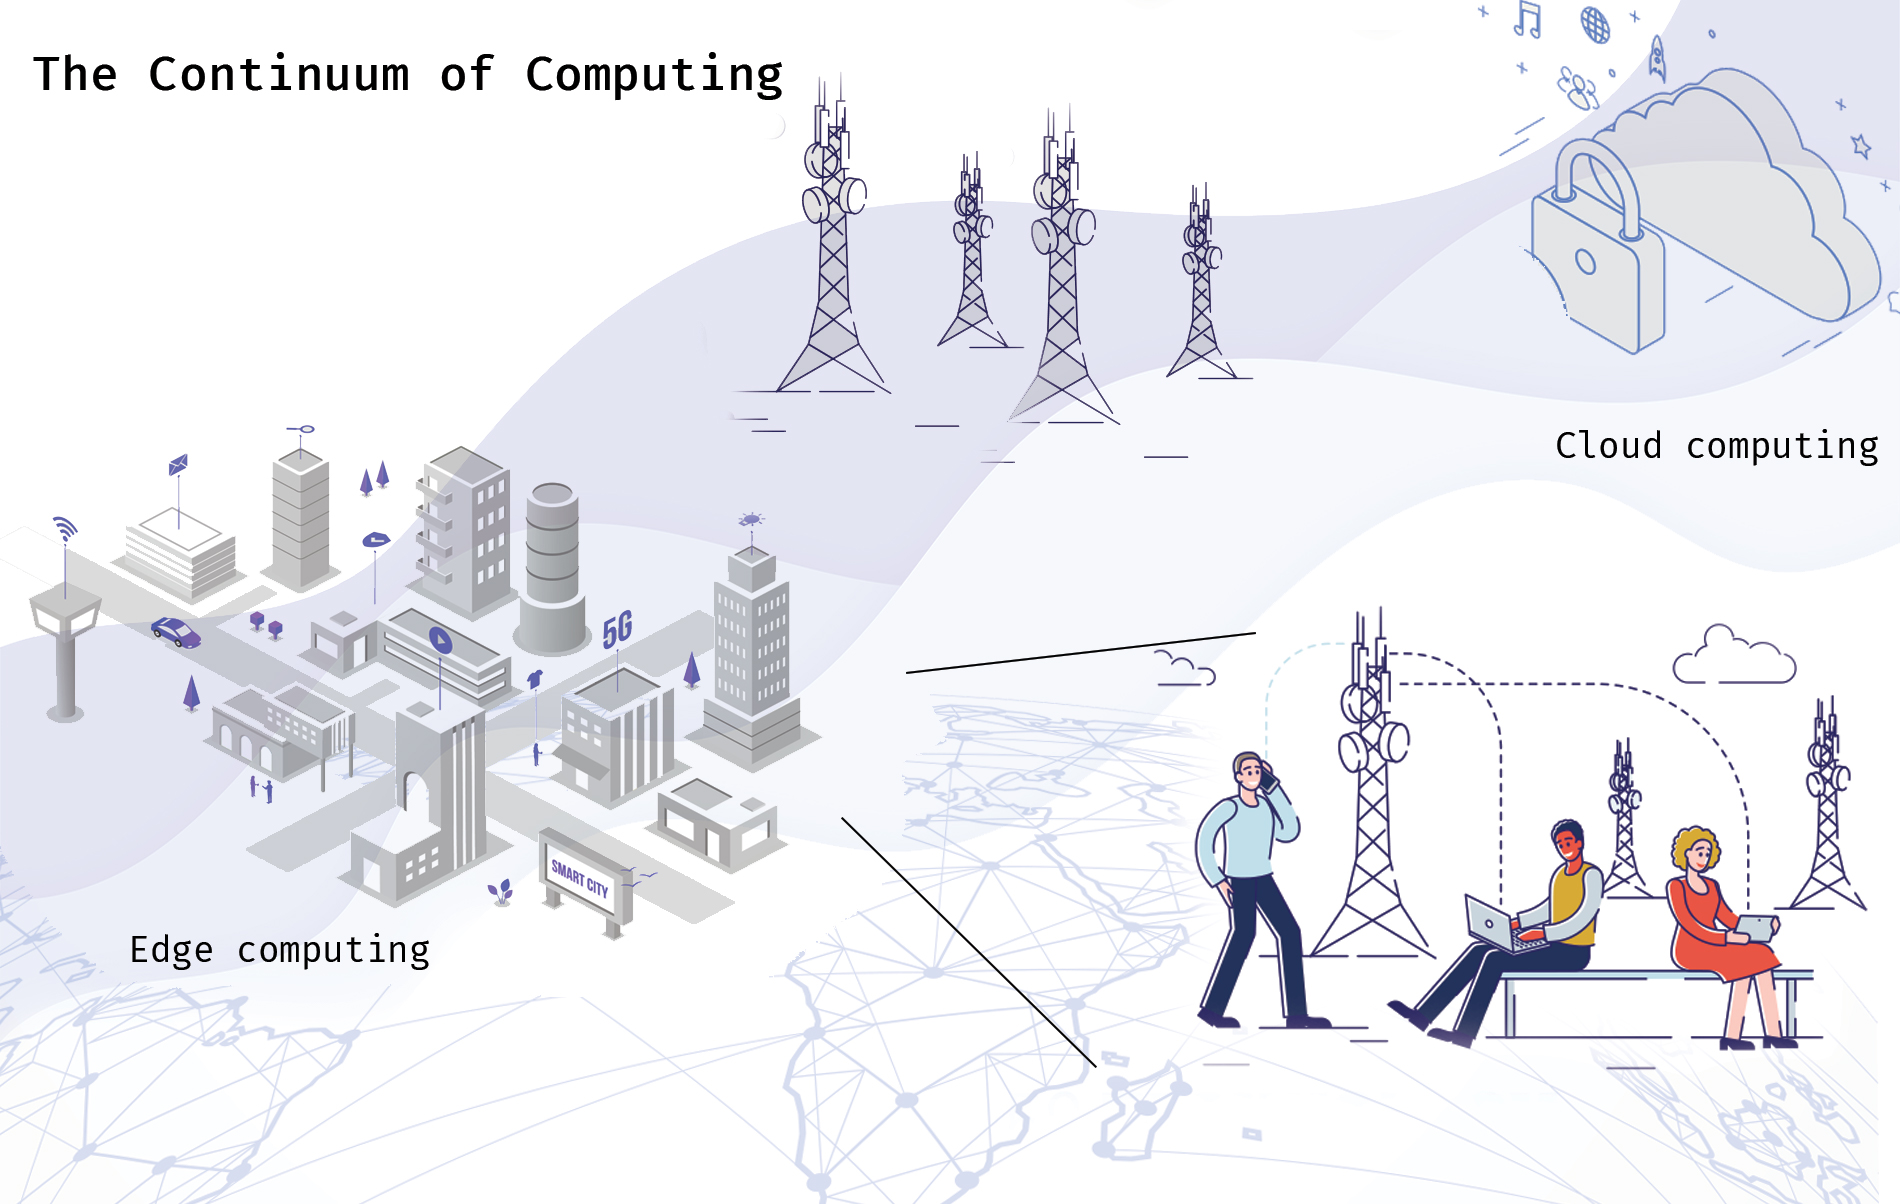
\includegraphics[width=\textwidth]{figures/continuum}
\caption{Pictorial view of the continuum of computing \label{fig:continuum}}
\end{figure*}

The Internet has evolved significantly since its inception. It has grown into a ubiquitous platform for everyday services from just a simple communication layer for information sharing between researchers. Many changes and infrastructure trends drive this transformation.

First, during the past decade, the sharing of server and networking capabilities - known as the cloud computing para\-digm - has become a reality, giving users and companies access to virtually unlimited amounts of storage and computing power. Nowadays, many constantly connected mobile devices, servers, and network components offer their virtualised capabilities to their users.

Second, as connectivity improved dramatically in affordability, bandwidth, reliability and reachability, people started bringing their devices with them and accessing the Internet anywhere and anytime, as shown in the bottom-right corner of Fig. \ref{fig:continuum}. This trend, in turn, boosted the evolution of mobile computing and led to the emergence of richer client-side web applications. The uptake of 5G connectivity will bring an even more massive boost to this trend. By the end of 2026, Ericsson estimates that over 3.5 billion people, or 45 per cent of the world's population, will have a 5G coverage subscription \cite{ericsson-5g}.

Nowadays, we are amid the so-called Internet of Things (IoT), where everyday objects (things) are connected to the Internet and each other. These "things" comprise a multitude of heterogeneous devices ranging from consumer devices, such as mobile phones and wearables, to industrial sensors and actuators \cite{chen2018edge}, smart transportation, grids \cite{mugarza2019dynamic}, and cities \cite{mitton2012combining} (represented on the right in Fig. \ref{fig:continuum}). There are two denominators of this diversity of devices. First, they operate at the leaf nodes of the Internet network. Second, they are "equipped with identifying, sensing, networking and processing capabilities that will allow them to communicate with one another and with other devices and services over the Internet to achieve some objective" \cite{whitmore2015internet}.

Thus, it is natural that as consumers, we want our Internet-capable devices (e.g., mobile phones, thermostats, electric vehicles) to adapt seamlessly to our changing lives and expectations, regardless of location \cite{beckman2020harnessing}.

% Besides, our capacity for collecting data is expanding dramatically. Nevertheless, our ability to manage, manipulate, and analyse this data to transform it into information and act upon it has not kept the pace \cite{abdelbaky2017computing}. Data sources and the size of the generated information are growing exponentially. They have outpaced the Internet ability to transport this data in a reliable and timely manner to the cloud. IoT applications demand a short response time, involve private data, and produce a large quantity of data which could be a heavy load for the network transport layer. Cloud computing and Internet infrastructure are not capable of supporting these applications and their exploding multitude.

Fig. \ref{fig:continuum} depicts a new vision, where the computing will converge to a pervasive continuum that seamlessly combines this data and computing power to model, manage and make use of virtually any realisable application of interest. Use cases exist in diverse application areas, from managing extreme events (e.g. environmental monitoring \cite{brzoza2016embedded}) to optimising everyday processes (e.g. manufacturing \cite{chen2018edge}) and improving life quality (e.g. healthcare \cite{pace2018edge} and smart cities \cite{he2017multitier}).

A natural requisite of this vision is that computational capabilities are gradually being introduced at the network's edge, where devices are connected to the Internet and communicate with each other, as represented by the smart city in Fig. \ref{fig:continuum}. This inter-communication constitutes the edge networks. New approaches that combine distributed services close to the data sources (i.e. edge nodes) with resources in the cloud and along the data path can establish a computing continuum and effectively process this data. Depending on the use case and service level requirements, user applications may require processing and storage locally (edge computing), in the cloud, or somewhere in between. Fog computing \cite{fog-computing} is the term coined by the research community to identify computational resources situated at a few, usually one, hop away from end-users. Fig. \ref{fig:continuum} represents the fog computing as base stations, to which users connect to in everyday activities.

% This trend lays the groundwork for novel and ubiquitous services in a wide range of application domains. To cite Haller et al. \cite{haller2008internet}, this paper believes that we are close to "a world where physical objects are seamlessly integrated into the information network, and where the physical objects can become active participants in business processes. Services are available to interact with these 'smart objects' over the Internet, query their state and any information associated with them, taking into account security and privacy issues."

This paper proposes a vision that follows naturally from the previous premises - the \textbf{continuum of computing} - a ubiquitous system where distributed on-demand resources and services on the whole computing continuum are dynamically provisioned to support different ranging services and released with minimal management effort.

There will be pervasive service platforms anywhere the user is and a multitude of services available over the Internet. The service providers will provide services, and consumers use them to accomplish any high-level application-specific goal. Services will be composed based on other existing services, leveraging the principle of reuse. These services' granularity will be very different, ranging from high-level business services to low-level sensor services provided by the Internet of Things.

It is fundamental that software and hardware provided as-a-service is a first-class citizen, allowing such services to be dynamically placed by decoupling them from their location. The continuum must also facilitate the elastic provisioning of virtualised end-to-end service delivery infrastructures. Virtual capabilities are leased, dynamically configured and scaled as a function of user demand and service requirements. End-to-end network configuration is a primary example of a virtual capability that needs to be scaled elastically according to the execution's dynamics. The continuum must behave as a fluid, which continuously adapts its shapes to fit the environment, as first described in \cite{latre2014fluid}. In Fig. \ref{fig:continuum}, the three spaces of computing (cloud, fog, and edge) are immersed in the fluid computing continuum, where computation can freely flow like a water droplet. This freedom of movement is an evolution to the common practice of merely connecting the network nodes to allow computation to happen at pre-determined locations in the computing space.

% However, this vision goes beyond the traditional elasticity of clouds. In addition to computational, network and storage resources, the managed capabilities include end-to-end network configuration, high-level service and device functionalities.

The notion of "the continuum of computing" is not entirely novel and has been anticipated before. The authors of \cite{latre2014fluid} envision a Fluid Internet, which "seamlessly provisions virtualised infrastructure capabilities, adapting the delivery substrate to the dynamic requirements of services and users, much like a fluid adapting to fit its surroundings". The researchers in \cite{abdelbaky2017computing} present the notion of computing in the continuum as well, as "a fluid ecosystem where distributed resources and services are programmatically aggregated on-demand to support emerging data-driven application workflows". Similarly, the authors of \cite{beckman2020harnessing} define the continuum of computing and seek to develop approaches that include the entire computing continuum as a collective whole.

The vision of continuum would not be feasible without the previous groundwork done in the research areas of cloud computing and IoT. These two topics have gained extreme popularity in the last decade. More recent works like \cite{botta2016integration} focus on integrating the cloud and IoT but keeping the two as distinct spaces where the latter sends data and offloads computation to the former. The few publications mentioned in the previous paragraph are the only ones to foresee a continuum of computing encompassing the whole Internet as a substrate for ubiquitous services. Unfortunately, however, to the best of the author's knowledge, very few efforts have been carried out on developing platforms to make this vision possible and optimised.

The remaining parts of this paper are organised as follows. Section \ref{sec:problem} discusses the present trends which lead to the continuum and \ref{sec:challenges} presents the challenges of this vision. Section \ref{sec:technicals} shows the problem space addressed by this paper and the technology baseline. Section \ref{sec:evaluation} contains an evaluation of the architecture presented in the preceding section and, lastly, the paper concludes in Section \ref{sec:conclusion} with the final remarks about the preliminary results of this work.

\section{Problem statement}
\label{sec:problem}

In the past decade and now more than ever, cloud computing \cite{mell2011nist} has provided users with the potential to perform computing tasks utilising resources physically distant.

% A popular definition of cloud computing \cite{mell2011nist} is "a model for enabling ubiquitous, convenient, on-demand network access to a shared pool of configurable computing resources (e.g., networks, servers, storage, applications, and services) that can be rapidly provisioned and released with minimal management effort or service provider interaction."

% The cloud architecture can be split into four layers: datacentre (hardware), infrastructure, platform, and application \cite{zhang2010cloud}. The resulting model is divided into three types of service: Infrastructure as a Service (IaaS), Platform as a Service (PaaS), and Software as a Service (SaaS). Accordingly, to the developers' needs, IaaS can be chosen if one wishes to customise every aspect of how an application gets deployed and executed, leaving the responsibility for provisioning the hardware or virtual machines to the cloud provider. Otherwise, in PaaS and SaaS, the developers have no control over the infrastructure but can access prepackaged components or complete applications, respectively. Thanks to such flexibility in the service layer, the cloud computing paradigm has been highly successful. By 2023, Gartner predicts that 40\% of all enterprise workloads will be deployed in cloud infrastructure and platform services, up from 20\% in 2020 \cite{gartner-cloud-edge}.

Conventional single provider infrastructures hosting cloud services offer undoubtedly many benefits (e.g. affordability, scalability, and efficiency) but not without challenges. A large data centre's energy consumption is high to keep it operational, and like any other centralised computing model, the issues resulting from sudden interruption would be adverse in terms of downtime cost.

Another issue of cloud-only solutions is that the required data must be transferred and stored in separate places from the source. Data centres are often geographically distant from the application users, notably when the data is generated at edge locations. However, the private exchange of sensitive or personal data is critical for many applications. For instance, in healthcare, data cannot be stored in the public cloud to ensure patient's privacy.

Besides, the evolution of the Internet of Things is having a significant impact on cloud computing generally, and it is exposing the limitations of the latter. The number of connected devices increases exponentially with estimations of dozens of billions of "things" going live in the coming years \cite{gartner-iot}.

As a consequence of connecting these "things" to the Internet, large volumes of data are being generated at unprecedented volumes, variety and velocity. This data is currently transferred and stored in the cloud in a centralised architecture. Data transfer, especially in these volumes, is costly in networking pricing (e.g. ingress traffic to the cloud and network transportation) and retards computational performance.

Thus, it becomes evident that traditional data processing methods where data is collected at the edge and processed in a central instance will not suffice. A more decentralised solution is required where data processing could take place before transfer and storage. The key is to reduce the number of messages and the amount of data transmitted throughout the continuum so that data should be processed locally or only where it makes sense.

With these premises, the rationale for achieving cloud-like capabilities in the continuum is two-fold. First, it offers on-demand virtual capabilities regarding storage, memory and processing units that augment IoT devices and components with limited computation capabilities due to form factors. Note, however, that fog and edge nodes cannot scale "infinitely" as cloud data centres do.

Second, scaling fog and edge infrastructure is arduous and time-consuming, even more as in cloud infrastructure, due to additional factors such as heterogeneity, network unreliability and difficulty to predict capacity needs in advance. Underprovisioning means potentially losing business, while overprovisioning means wasting money on unused infrastructure \cite{nygren2010akamai}.  Moreover, user demand at the edge can be very often spiky \cite{nygren2010akamai}, meaning that companies would need to provision for anomalous peaks like gatherings and events, investing in significant infrastructure that sits underutilised most of the time. Overprovisioning also has an environmental cost when underutilised infrastructure consumes significant amounts of power.

The cloud computing model applied to the fog and edge as services is attractive since it allows businesses to decrease the required capital expenditure and frees them from the need to invest in infrastructure. Businesses can rent resources according to their needs and only pay for the usage \cite{botta2016integration}. Moreover, it reduces operating costs, as service providers do not have to provision capacities according to maximum peak load. Resources are released when service demand is low.

On the other hand, the cloud can benefit from the fog and edge by extending its scope to reach real-world things in a more distributed and dynamic manner and delivering new services in a large number of real-world scenarios. Such an extension will impact future application development, where this new flow of information gathering, processing, and transmission will generate new challenges (described in Section §\ref{sec:challenges}).

\subsection{Decentralization}

Consequently, highly distributed networks are the most effective architecture for the continuum, particularly as services become more complex and more bandwidth-hungry. Although often referred to as a single entity, the Internet is actually composed of a variety of different networks. The net result is that content generated at the edge must travel over multiple networks to reach its centrally hosted data centre.

Unfortunately, inter-network data communication is neither an efficient nor reliable operation and can be adversely affected by a number of factors.

\begin{figure}[ht]
\centering
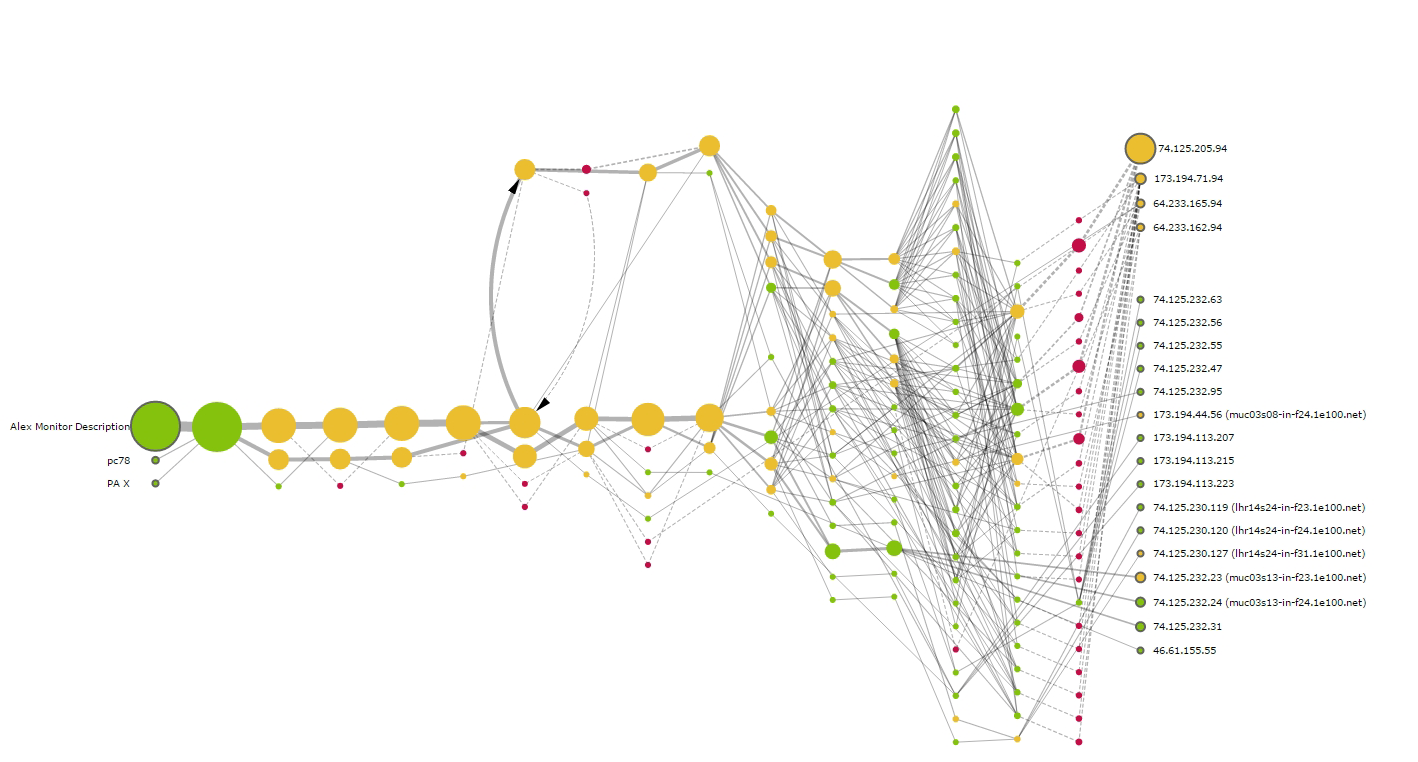
\includegraphics[width=\columnwidth]{figures/traceroute}
\caption{Traceroute virtualisation of an IP packet reaching google.com \label{fig:traceroute}. The left green nodes are the source nodes and the packets travel throught to the extreme right, where servers are located in datacentres. Source \cite{traceroute-google}.}
\end{figure}

The peering points, depicted nodes in Fig. \ref{fig:architecture}, are where networks exchange traffic and are the common bottleneck of the Internet. Capacity at these points typically lags behind the reliability demand mainly due to the economic structure of the Internet \cite{nygren2010akamai}. The economic incentive flows in at the first mile (cloud data centres) and at the last mile (IoT), with however very little interest to invest in the middle network composed of peering points. These points thus become the cause for packet loss and increased latency.

Across the Internet, outages are happening all the time, caused by a wide variety of reasons such as cable cuts, misconfigured routers, DDoS attacks, power outages, or even earthquakes and other natural disasters. While failures vary in scope, large-scale occurrences are not uncommon \cite{aws-outage}.

When dealing with a pervasive system such as the continuum, it is no longer sufficient to simply have enough server and network bandwidth resources. One must consider the throughput of the entire path from IoT devices to data centres to end-users. The bottleneck is not likely to be at just the extreme ends of the path. It could be at a peering point, as mentioned, or due to the network latency between server and device. 

Autonomous vehicles are an evident example of these issues. One Gigabyte of data will be generated by autonomous cars every second, and they require real-time processing for the vehicle to make correct decisions \cite{shi2016edge}. Such a situation can quickly challenge the network bandwidth and reliability to support many vehicles in one area. Moreover, if all the data were to be sent to the cloud for processing, the response time would be too long. In such cases, the data needs to be processed at the edge for shorter response time, more efficient processing and lesser network pressure.

Secondly, in many other cases like environmental monitoring, most of the end nodes in IoT (e.g. sensors and actuators) are energy-constrained things, so offloading some computing tasks to the edge could be more energy efficient. Even mobile phones benefit significantly from reduced energy consumption, especially for tasks like Mobile Augmen\-ted Reality \cite{baresi2017empowering}.

For these reasons, alternate models such as fog computing \cite{fog-computing} and edge computing \cite{shi2016edge} have emerged in recent years. Such computing models arise from the general idea of processing the information at the nearest spot. A fog and edge-based platform, with servers anywhere the end device, can achieve the scale needed as well. Each location supports higher orders of throughput, low response times, and higher energy efficiency.

However, information processing at the nearest physical node may not always be a good option. If the task requires long computation, as in big-data analysis, it will be better to offload to the more capable but distant node till the cloud at the opposite extreme point. A request's latency is the sum of two components: the computing latency and the transmission latency. High computing latency can outweigh transmission efficiency. Therefore, edge computing has the responsibility to determine the ideal tradeoff between computing latency and transmission latency, leveraging resources on the whole continuum to achieve the best optimisation on a case-by-case basis.

Similar attention must be dedicated to the energy issue. The battery is the most precious resource for things at the edge of the network, but the wireless communication module is usually very energy-hungry \cite{shi2016edge}. For a given workload, it is not always the case that the most energy-efficient solution is to offload the whole workload to the edge rather than compute locally. The key is the tradeoff between computation energy consumption and transmission energy consumption. Offloading to another node is preferable only if the latter overhead is more negligible than computing locally.

Such dynamism to determine the best location for the computation to happen is a proof that the vision of a computing continuum requires a seamless movement of information and computation. Besides, the computing continuum is not one form of computing (e.g. edge computing) supplanting another (e.g. cloud computing), but an evolution to harness the entire computing space as a whole.

% Some trending computing models relevant to the decentralisation above are now presented.

% \subsubsection{Fog Computing}

% Fog computing \cite{fog-computing} is a decentralised computing infrastructure that is used mainly as a complement to cloud computing. It leverages the compute resources at the edge network and brings the computational processing closer to the data source by offloading workload to edge nodes from cloud data centres. The network nodes near the edge providing these resources are called fog nodes, and they are usually a single hop away from the end-users. An example of such nodes is the base stations depicted in the bottom-right illustration in Fig. \ref{fig:continuum}.

% Overall, any device with computing, storage, and network connectivity can constitute a fog node. Examples include switches and routers inside buildings (pictured in the smart city in Fig. \ref{fig:continuum}), industrial controllers, embedded servers and video surveillance cameras \cite{jang2018application}. In recent years, the spread of fog computing has been facilitated by the availability of suitable hardware in small, affordable, low-power computers (e.g. Raspberry Pi \cite{raspberry}).  Improvements in virtualisation technologies that enable slicing resources between different users to provide isolated environments (see Section §\ref{sec:virtualisation}) have also helped.

% The Cloudlet \cite{satyanarayanan2009case} architecture is one of the first approaches that offer an example of fog computing with virtual machine (VM) techniques. Its computing power is much less than a conventional cloud infrastructure as cloudlets are composed of less powerful processors and are significantly smaller in size.

% \subsubsection{Mobile Edge Computing}

% Edge computing \cite{shi2016edge} denotes any computing and network resource that is located only at the extreme edge of the network. The rationale of edge computing is that computing should happen in the proximity of data sources, thus ideally \emph{at} the data source, eliminating the costly data transfer to a remote data centre. The result significantly improves Quality of Service (QoS), similar to fog computing, and the end-user earns considerable network latency reduction and bandwidth consumption.

% When the end-users are mobile devices, edge computing is referred to as mobile edge computing (MEC) \cite{beck2014mobile} as well. In contrast to the broader term edge computing, MEC focuses on co-locating computing and storage resources at base cellular networks stations. Being co-located at base stations, MEC servers' computing and storage resources are available close to mobile users like smartphones and smart vehicles and can support mobility between cellular cells. MEC is seen as a promising approach to increase the quality of experience in cellular networks and a natural direction for the evolution to 5G networks \cite{yousaf2017nfv}.

% \subsubsection{Serverless Computing}

% Serverless computing \cite{jonas2019cloud} involves building, running and providing applications and services without considering the server-side. "Serverless" does not mean that there is no server usage, but rather that the application developers focus on the application itself rather than what happens on the physical infrastructure.

% Serverless computing is synonymous with Function-as-a-Service (FaaS) and event-based programming as underlying provisioning and instantiation of the resources will happen only when necessary and not all the time. Notably, provisioning happens on the fly when an event triggers the execution of a function. In particular, FaaS triggers a server's infrastructural provisioning only when a function is requested, then executes the expected operations and frees the resources above as soon as they are deemed to be not necessary.

% The major benefits of this model for cloud consumers are increased scalability and applications' infrastructure independence, and lower costs. Similarly, cloud vendors also have strong incentives for services to be built on serverless architectures as opposed to following a fixed-price model for long-running VMs. VM deployments tend to be very static as users deploy them for long periods. In contrast, the FaaS computing model tends to offer more variation in memory and CPU utilisation. As a result, the serverless computation gives a better opportunity to optimise resource usage and bill users for function invocation and network utilisation.

% Recently, the leading cloud vendors (e.g. Amazon and Microsoft) are putting effort into making it easier to integrate edge functionality into their clouds, mainly by providing serverless computing and tight integration with their other cloud services. As an example, AWS Lambda@Edge \cite{aws-lambda-edge} allows using serverless functions at the AWS edge location in response to CDN event to apply moderate computations. On the other hand, AWS Greengrass \cite{aws-greengrass}, and Azure IoT Edge \cite{azure-iot-edge} are commercial solutions specifically targeting serverless for IoT.

% Recent works in the literature have argued the advantages of edge computing too. An instance, the authors of \cite{baresi2017empowering} present an augmented reality use case for mobile edge computing, in which computation and data-intensive tasks are offloaded from the devices to serverless functions at the edge, outperforming the cloud alternative up to 80\% in terms of throughput and latency.

\section{The challenges ahead}
\label{sec:challenges}

% After discussing the decentralisation trend, this section presents the challenges in implementing such a vision. As an example, the heterogeneity of the connected devices is immense. It can be seen from different perspectives, such as computing performance, storage and network requirements, communication protocols, energy consumption, to name just a few. Such diversity poses questions about handling the virtualisation of the underlying resources and the nodes' interoperability. Both challenges are explored in Section §\ref{sec:virtualisation} and §\ref{sec:interoperability} respectively.

To enable the continuum, this paper identifies the following challenges as important ones to be addressed. The list should not be considered exhaustive by any means, nor the most significant ones. Dynamic network configuration and distributed persistent storage are two examples of critical technical challenges, which the author has not explored yet in his work.

Besides being characterised by very high heterogeneity, the edge lacks important features such as service orientation, interoperability, orchestration, reliability, efficiency, availability, and security. Therefore, it is natural that many challenges in the continuum's realisation overlap with open research problems in edge computing. At the same time, other issues are originated, or at least exacerbated, by the desire for holistic integration of cloud, fog, and edge computing.

% \begin{enumerate}
%     \item \emph{Context-sensitive service orientation}: as stated in the introduction of this paper, services must be treated as first-class citizens, allowing them to be dynamically placed and decoupling them from their location. Consumers should only be concerned with what they want to do and accomplish and providers with how that could be done and provided to the user. At the same time, services need to be aware of different aspects of the environment they are acting in, whereas today's services are rarely context-sensitive;
%     \item \emph{Orchestration}: advanced orchestration systems are required to support the resource management of heterogeneous devices and be adapted to many applications running on the edge connected devices;
%     \item \emph{Virtualisation}: the system has to provision resources and provide access to heterogeneous IoT resources and hardware such as GPUs. Besides, today's common practice in the cloud assumes enumerated resources and predictable computing capabilities. However, in the continuum, the capabilities and numbers of components change dramatically over time and require virtualisation solutions to provide a reliable service. \linebreak Lastly, edge computing must support multi-tenancy, and the virtualisation techniques are likely to be asked to deliver execution environments even more hardened than in cloud centres;
%     \item \emph{Dynamic configuration}: dynamic configuration on constrained devices would allow them to actively participate in the continuum and dynamically adapt to environmental context changes based on the application requirements. The benefits are increased accuracy in machine-learning predictions, lower response times and more flexible data transformation at the data source;
%     \item \emph{Interoperability}: applications on a continuum should be able to amalgamate services and infrastructure from different locations seamlessly. Every node on the Internet should additionally expose a uniform interface to its resources and services;
%     \item \emph{Portability and programmability}: developers should be provided with the languages and tools to program applications and services to run in such a dynamic environment without having to reinvent themselves;
%     \item \emph{Mobility}: efficient migration of each application and service has to be supported from platform to platform and to follow the users' movements in the network (roaming);
%     % \item \emph{Reliability}: services in the continuum could fail due to various reasons, notably at the edge. The establishment of reliable communication between nodes must be supported;
%     \item \emph{Security and Privacy}: personal and sensitive user data are subjected to high risk while many users access Internet services from anywhere. Security and privacy matter even more when personal data may have to be stored closer to the users/devices to facilitate computing and processing on the edge or fog layer.
%     % \item \emph{Energy efficiency}: obtaining energy efficiency in both data processing and transmission is an important open issue;
% \end{enumerate}

\subsection{Context-sensitive service orientation}

This paper envisions service-oriented paradigms as necessary for organising and utilising distributed capabilities that may be under the control of different ownership domains. A Service-Oriented Architecture (SOA) provides "a uniform mean to offer, discover, interact with and use capabilities to produce desired effects consistent with measurable preconditions and expectations" \cite{mackenzie2006reference}.

According to this model, the major components of a basic SOA and their possible interactions are constituted by a service provider that publishes its service interface (how other services access their functionalities) via a service registry where a service requester/consumer can find it and subsequently bind to the service provider \cite{haller2008internet}.

The SOA reference model's central concept lies in services that provide access to capabilities to be exercised by following well-defined interfaces and a service contract with constraints and policies. This enables the loose coupling of services and minimisation of mutual dependencies.

Services are provided by the service providers and used by others, the service consumers, a role usually taken on by application developers. Services may be composed based on other existing services, thereby adhering to the principle of reuse. They are responsible only for the logic and information they encapsulate, uniformly described and publicly retrievable via service discovery mechanisms. This design is in net contrast to today's practice. We continue to build ad-hoc programs confined in single points of the continuum, defining individual device computing behaviours \cite{beckman2020harnessing}.

However, to enable the seamless and agile interoperation of services in the continuum, several challenges still exist concerning their organisation and implementation.

First of all, the lack of neutral, trustworthy and widely accepted service intermediaries on the Internet of today still prevents establishing the continuum described above. Service intermediaries are necessary to facilitate the efficient retrieval of services that match a given user need and provide service performance by monitoring service quality and availability. Unfortunately, so far, single cloud providers such as Amazon Web Services, Google Cloud Platform or Microsoft Azure have shown no interest in inter-cooperation \cite{grozev2014inter}.

Secondly, the lack of means of composing higher-order services from various services imposes additional challenges to the emergence of the computing continuum. The lack of interoperability prevents services from being set up quickly and easily. Cloud providers and their respective systems adhere to different conventions with respect to interfaces and communication protocols. For instance, Google Cloud Platform services heavily use Protocol Buffers \cite{protobuf} in the services' APIs, a Google technology for serialising structured data. For this reason, a significant effort will be required to uniformly provide the service semantics and interfaces in a comprehensible way for both humans and machines. For example, the system would need to map high-level descriptions to vendor-specific implementations (e.g. "key-value store" would map to different AWS or Google Cloud products).

Lastly, services on the Internet of today can be considered mute and unresponsive. In the future, services are expected to become communicative and reactive to their respective environments, particularly in two respects \cite{haller2008internet}. Existing service interfaces (e.g., REST-based) are not yet designed to be interpreted and used by machines but rather by humans. This issue frequently prevents the systems from easily discovering and interacting with them. Methods are needed to improve both user-service interaction and machine-to-machine communication. Today's services are clearly built with human interaction in mind. Fortunately, recent REST community efforts are trying to compensate for the lack of M2M communication \cite{openapi}.

% \subsubsection{Service-oriented architectures}

% The idea of service orientation can be partially traced back to the object-oriented programming (OOP) literature \cite{dragoni2017microservices}. However, the evolution of objects into services, and the relative comparisons, has to be treated carefully since the first focus on encapsulation and information hiding in a shared-memory scenario. In contrast, the second is built on the idea of independent deployment and asynchronous communication via well-defined interfaces. However, both paradigms share the common idea of componentisation.

% The last decade has seen a further shift towards the concept of service first and the natural evolution to microservices afterwards. SOA has been introduced to harness distributed systems' complexity and integrate different software applications. In SOA, a service offers functionalities to other components, accessible via message passing. Services decouple their interfaces from their implementation.

% This design is in striking contrast to monolithic architectures, where the application is composed of a single program, typically providing a user interface and data access through a database. However, monolithic architecture poses real challenges and difficulties when growing exponentially because of the need to scale up \cite{dragoni2017microservices}.

% SOA is built around services designed to work in an orchestrated manner to modularise the system. It is more challenging to divide the application into multiple services, but it enables greater flexibility, extensibility and reusability of existing services for multiple use cases. The model's benefits are application modularity and service reusability \cite{lynn2020cloud}, which are both very important to enable a computing continuum. However, a major disadvantage is the complexity of orchestrating and monitoring all the services and the underlying infrastructure, especially when the project is complex and the components' amount is huge.

% The first generation of SOA architectures defined daunting and nebulous requirements for services (e.g., discoverability and service contracts) \cite{dragoni2017microservices}, which hindered the adoption of the model. Microservices are the second iteration, introduced as a solution for the gaps in the SOA approach.

% The microservices approach divides applications into more granular components by distributing them into small self-contained services. Each service implements and attends to separate business functions and capabilities to maintain independence from other services. They are mainly deployed in an automated manner, through a container (more on that in §\ref{sec:virtualisation}), and communication happens through REST APIs \cite{rest}, therefore making the impact of the programming language insignificant.

In terms of the continuum, a SOA realised through the \emph{as-a-service} model allows consumers to be only concerned with what they want to do and accomplish, and providers with how that could be done and provided to the user. A successful interface establishment between those two actors can lead to minimal direct consumer interaction with the provider's infrastructure, allowing complete control to the provider and no cost of ownership for the former.

\begin{figure}[ht]
\centering
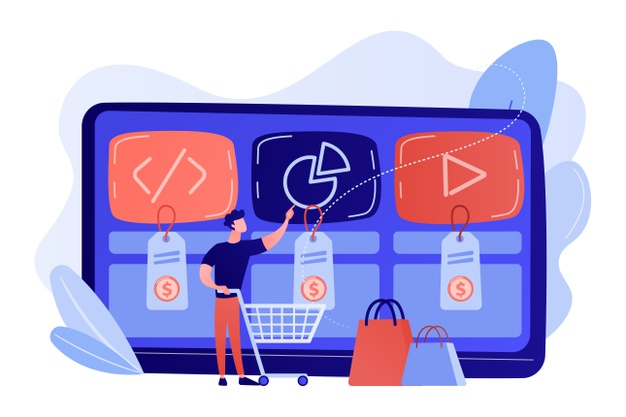
\includegraphics[width=\columnwidth]{figures/marketplace}
\caption{A digital service marketplace \label{fig:marketplace}.}
\end{figure}

Furthermore, this architecture results in a system where various service implementations should already exist, maybe provided in the same fashion of a service marketplace (e.g. Shopify App Store \cite{shopify}). Fig. \ref{fig:marketplace} is a picture of such a digital service marketplace, where consumers can use not only Software-as-a-Service products like YouTube but also define their applications. The consumer himself does not have to be an expert and may use high-level languages to specify requirements, constraints and workflow to achieve arbitrary goals. Even the infrastructure's physical resources should not be consumer-aware, and there may be several diverse implementations to meet specific service demands. These implementations can differ in hardware type or service level requirements and could be characterised by different price and performance attributes.

Lastly, today's web services are rarely context-sensitive. However, to support context-sensitive services at the edge, they need to be aware of different aspects of the environment they are acting in. Context services can provide such information to the application services that implement local control loops and trigger specific actions based on context events. Such context services can be composed of lower-level services which deliver individual sensor readings.

% On this matter, the MEC architecture provides the advantage of data locality, which lets a given application store the context data only regarding the devices within the region covered by the base station. Such an advantage is two-fold: providing location-aware services is more accessible, and less data has to be persisted in each zone. For example, MEC servers in \cite{baresi2017empowering} can retrieve the machine learning features in an augmented reality scene, match them against a local database, and return the corresponding data (information about monuments, buildings and other points of interest) to the client application.

\subsection{Orchestration}

The transition to the continuum will require coordinating and scheduling the operation of a myriad of distributed service components, whose complexity makes the necessity of service orchestration paramount. Besides, it will also be a crucial feature for many IT organisations and DevOps adopters to speed the delivery of services, simplify optimisation, and reduce costs \cite{nygren2010akamai}. However, the continuum's orchestration is challenging due to the scale, heterogeneity, and diversity of resource types and the uncertainties of the underlying environments. The uncertainties arise from a number of factors, including resource capacity demand (e.g. bandwidth and memory), failures (e.g. failure of a network link), user access pattern (e.g. the number of users and location) and lifecycle activities of applications.

Another difficulty caused by the underlying resources' heterogeneities is providing proper pricing models that take into account locations, resource types, and sizes. Considering such variables would enable, for instance, to dynamically provision resources of different pricing models to the cluster to satisfy application-specific needs with minimum cost.

Generally speaking, orchestrating the services in the continuum is a considerable challenge. It encompasses different technologies from different fields, including, among others, wireless cellular networks, distributed systems, virtualisation, and platform management. It imposes new interaction models among different heterogeneous clouds and requires mobility handover and migration of services at both local and global scales.

\subsection{Virtualisation}
\label{sec:virtualisation}

The rapid pace of innovation in data centres and software platforms has transformed how companies build, deploy, and manage online applications and services. The high costs of buying and maintaining large numbers of machines, and the fact that each was often under-utilised, led to a great leap forward in virtualisation.

Virtual Machine Monitors (VMM) \cite{rosenblum2005virtual} were born at the end of the 1960s as a software abstraction layer that partitions a hardware platform into one or more virtual machines (VM) to run existing software unmodified. Nowadays, however, a VMM is more a solution for security and reliability.

% Functions like migration and security, which are difficult to achieve in modern operating systems, seem much better suited to implementation at the VMM layer. KVM (Kernel-based Virtual Machine) \cite{kvm} is an example of VMM built into the Linux kernel that allows a host machine to run multiple, isolated virtual machines. 

On the contrary, Linux Containers (LXC) \cite{bernstein2014containers} are an OS-level virtualisation method for running multiple isolated applications sharing an underlying Linux kernel. A container consists of one or more processes with reduced privileges, having restricted visibility into kernel objects, and host resources.

With containers, applications share an OS. As a result, these deployments will be significantly smaller in size than VM deployments, making it possible to store a few thousand containers on a physical cloud host (versus a strictly limited number of VMs). Adopting containers can ideally lead to a future where the end-user can deploy services and applications on edge computing platforms on heterogeneous devices with minimal effort. Several works in literature (e.g. \cite{pahl2016container} and \cite{bellavista2017feasibility}) have argued the feasibility of container virtualisation applied to cheap low-powered devices, namely the Raspberry Pi \cite{raspberry}.

Containers provide resource isolation, self-contained packaging, anywhere deployment, and easiness of orchestration. All these features make containers a very compelling technology for the continuum.

To be precise, however, many of these characteristics are a merit of the underlying Docker image technology \cite{docker-image} rather than the container virtualisation per se. Images package applications with individual runtime stacks, making the resultant software independent from the host operating system. This self-containment makes it possible to run several instances of an application on different platforms. Many leading cloud providers like Amazon, Google, Microsoft, IBM and others use this technology for enabling Platform-as-a-Service and Function-as-a-Service.

Existing serverless \cite{jonas2019cloud} platforms such as Google Cloud Functions \cite{gcloud-functions}, Azure Functions \cite{azure-functions} and AWS Lambda \cite{aws-lambda} isolate functions in ephemeral, stateless containers. However, the use of containers as an isolation mechanism causes latencies up to hundreds of ms or even 5 seconds \cite{mohanty2018evaluation}, which are unacceptable for latency-sensitive services operating ad the edge. These platforms cache and reuse containers for multiple functions call within a given time window, notably 5 minutes, to achieve better efficiency. Similarly, some users send artificial requests to keep the containers alive. In the edge environment, the long-lived and over-provisioned containers can quickly exhaust the limited node resources and become impractical for serving many IoT devices. Therefore, supporting a high number of serverless functions while providing a low response time (say 10ms \cite{elbamby2019wireless}) is one of the main performance challenges for resource-constrained edge computing nodes.

In addition to the latency matter, containers have a not negligible resource footprint and isolation issues. Containers offer relatively weak isolation to the point where containers are run in per-tenant virtual machines to achieve proper isolation. Unfortunately, virtual machines' resource requirements are too demanding for the edge or fog nodes. A light\-weight yet robust isolation solution is, therefore, a hot research question.

Accordingly, recently lightweight isolation platforms have been introduced as a bridge between containers and full system virtualisation. Both Firecracker and gVisor \cite{caraza2020blending} rely on host kernel functionality. Firecracker provides a narrower interface to the kernel by starting minimalistic guest VMs and providing full virtualisation, whereas gVisor has a wider interface. They both have low overhead in terms of memory footprint, in any case. For instance, Amazon Firecracker has a memory footprint of 5MB and startup latency of about 125ms \cite{firecracker}.

Lastly, it is worth mentioning that Unikernels \cite{madhavapeddy2013unikernels} are another novel virtualisation technique. Unikernels comprise a minimal operating system and a single application, making them a natural alternative to containers. Unikernel-based serverless experiments yield at least a factor of 6 better latency and throughput than mainstream solutions \cite{koller2017will}. Unikernel implementations lack the maturity required for production platforms, e.g. missing the needed tooling and a way for non-expert users to deploy custom images. This disadvantage makes porting containerised applications very challenging. Besides, container users can rely on a large ecosystem of tools and support to run unmodified existing applications.

As a concluding note, the basic units of execution have continuously shrunk in the past years: from VMs to containers and serverless functions (at least in a virtual sense, as serverless functions are currently built into vendor-specific container images behind the scenes). Such smaller execution units are dictated by the need for increased flexibility execution environment and strong economic incentives to increase resource utilisation. Consequently, applications are increasingly becoming comprised of distributed components, and the number of lines of code associated with each unit of execution has dramatically decreased.

\subsection{Dynamic configuration}

Edge systems and IoT nodes must promptly recognise the environmental context changes under which they are subject. Such changes are often critical to many applications like video analysis \cite{jang2018application}. This failure is because the service controller running on the edge can validate the data's usefulness (e.g. video frame) only after receiving the devices. Meanwhile, the IoT device will continue to perform poorly (or even uselessly) until the controller makes adjustments.

Dynamic configuration on constrained devices would allow dynamically adapting to environmental context changes based on the application requirements. This goal is usually achieved by running an application-specific computation on the node itself. The net result is a significant improvement in task accuracy (e.g. object detection), computational cost, and response time.

At the same time, opening the edge devices to arbitrary code execution exposes the system to malicious intents, meaning that even a single buggy line of code can lead to system compromise, threatening the controlled physical assets and potentially human safety. Current software isolation stacks are complicated to use in trustworthy embedded systems as the machine might lack the necessary hardware (e.g. Memory Protection Units), have insufficient memory or missing the required software (e.g. Linux kernel functions to operate containers). 

Hardware support is often used to isolate non-embedded applications from each other and the OS from applications \cite{peach2020ewasm}. Dual-mode protection enables the kernel code to be inaccessible from applications at the cost of requiring mode transitions. In addition, Memory Protection Units (MPUs) enable the partitioning of memory into subsets, each accessible by separate applications. 
On the other hand, MPUs require OS, hardware, and build-system support. Thus the adoption of hardware memory isolation has been limited in microcontrollers as they typically lack the former two requirements.

A further challenge of IoT devices' dynamic configuration is allowing isolated execution with an acceptable compromise in efficiency loss and energy consumption. A common memory-safe execution technique is adopting interpreted languages (notably Lua) that provide type safety and ensure that all memory accesses adhere to the proper data type. Thus, memory accesses are constrained only to memory provided by the language runtime, usually via an interpreter, and are prevented from corrupting the device. For instance, the authors of \cite{brzoza2016embedded} have ported interpreters of high-level languages (Lua and Python) to C as a means to support dynamic reconfiguration of the internal logic in telemetry sensors.

% As an alternative, Software Fault Isolation (SFI \cite{wahbe1993efficient}) techniques provide memory safety instead by constraining loads and stores to a sandbox. When this data sandboxing is paired with control flow integrity (CFI), which ensures that execution can only follow paths intentionally generated by the compiler, the application's execution and memory accesses are constrained to the sandbox. Unfortunately, both the overheads of interpreting in the language runtime and performing the necessary memory checks in SFI are a concern, given the limited resources of microcontrollers.

\subsection{Interoperability}
\label{sec:interoperability}

There are and will be many different technologies for connecting and integrating all the things into the continuum. For example, ZigBee, IPv6 over Low-Power Wireless Area Networks (6LoWPAN), MQTT and CoAP \cite{naik2017choice} are all gaining popularity in the wireless sensor networking area, and OPC \cite{gruner2016restful} is well accepted in factory automation. However, the technologies are too different from expecting any standard to be able to cover them all.

For this reason, dealing with heterogeneity when building the continuum's edge infrastructure is necessary. Standards are undoubtedly helpful but will be hardly achieved. The key is to separate the functionality from its technical implementation, thus asking for interoperability instead of standardisation. Service-oriented architectures are ideal because they encapsulate functionality in services with a common interface, abstracting from the underlying hardware and protocols.

Having an infrastructure that allows connecting and integrating a diverse set of technologies is not just a "necessary evil" but rather a strength since it offers two key benefits. First, it allows for applying different solutions to different applications. Depending on the application requirements, the best-fitting technology can be used.

Secondly, an infrastructure where diverse technologies can easily be integrated into will be more future-proof. Especially in edge computing and IoT, the technical developments are not complete, and we can expect that new technologies and protocols will arise. An infrastructure built with technology diversity in mind will allow interoperability with existing and already deployed devices and networks.

With that said, cloud platforms heterogeneity is a non-negligible concern as well. Cloud services typically come with proprietary interfaces, causing resource integration to be adequately customised based on specific providers. This issue can be exacerbated when services in the continuum can depend on multiple providers to provide the different resources an application may require or to improve application resilience in case of single-provider failure \cite{grozev2014inter}.

Overall, cloud, IoT services, and applications are nowadays typically conceived as isolated vertical solutions. All system components are tightly coupled to the specific application context or the cloud provider. The interoperability challenge involves several aspects, where solutions need to be investigated in terms of uniformly access to cloud services \cite{grozev2014inter}, programming interfaces, and means for coping with data diversity.

\subsection{Portability and Programmability}

In cloud computing, users program their code and deploy them on the cloud. The cloud provider is the one in charge to decide where the computing is conducted in a cloud. Users have only partial knowledge of how the application runs. This easiness is one of the benefits of cloud computing: the infrastructure is transparent to the user. Usually, the program is written in the programming language the developer is most familiar with and between a limited selection (e.g. JavaScript, Java, Python, .NET). The application is then compiled for a specific target platform (typically x86\_64 GNU Linux) since the program only runs in the cloud.

As mentioned before in Section §\ref{sec:virtualisation}, cloud developers typically use containers spawned from images that include everything needed to run them. This package includes code, libraries, settings, and system tools. More importantly, these images can be constructed from minimal filesystem layers, and read-only layers can be shared, notably the base OS layer. Images hence are lightweight and use considerably less space than VMs. They offer benefits to developers in terms of ease of deployment, testing, and composition. Notably, they can be used to capture a development environment known to work for each application revision and share this environment among a team of developers. Organisations are widely using containers to deploy their increasingly diverse workloads to the cloud datacentres.

However, in edge computing and, by extension, in the continuum, the nodes have diverse platforms. The diversity of CPU architectures (namely x86\_64, ARM32, ARM64, and RISC-V) give programmers a hard time compiling for the different platforms. The nodes' runtime differs from each other, and the programmers face considerable difficulties in writing a service that may be deployed in the continuum paradigm.

Docker images attempt to overcome this issue by defining multiple variants (usually referred to as tags in Docker terminology) of the same image to target multiple architectures. A single image may contain variants for different architectures or even for different operating systems, such as Windows. Most of the official images on Docker Hub \cite{docker-hub} provide a variety of architectures. For example, official images usually support amd64, arm32v5, arm32v6, arm32v7, arm64v8, i386, ppc64le, and s390x. Despite this feature, a significant pain point is that developers are still required to configure and build their applications multiple times for each platform. Moreover, the absence of an OS on embedded devices or the limitation on resource capacity block any hope of running containers on such machines, mining the idea of containers as a unified solution for portability in the continuum (at least in their conventional form).

The theme of portability is often strongly connected to programmability. Making the proper technological choices (e.g. the programming language) is necessary to grant portable execution. To address the programmability in the context of edge computing, the authors of \cite{shi2016edge} propose the concept of computing stream defined as a serial of functions applied to the data along the data propagation path. Likewise, the work in \cite{beckman2020harnessing} proposes to use a simple Function-as-a-Service abstraction to program the continuum so that new algorithms and deep learning models can be pushed to appropriate locations (i.e., edge, fog, cloud, or HPC computing resources).

Serverless architecture naturally solves two critical problems for portability and programmability \cite{yi2017lavea}. First, the serverless programming model dramatically reduces users or developers' burden in developing, deploying, and managing applications. There is no need to understand the complex underlying procedures and distributed systems to run the applications. Second, the functions are flexible to run on either edge or cloud, which helps achieve the desired portability.

However, in this paper's view, the serverless computing model can satisfy only a limited subset of services, notably those with event-driven and request-reply nature. However, a common type of application is long-running services that require high availability and must handle latency-sensitive requests. Examples include user-facing service or industrial control loops. Another type of application is batch jobs, which have a limited lifetime and are more tolerable toward performance fluctuations. Examples include scientific computations or MapReduce jobs \cite{condie2010mapreduce}. Batch jobs are more suitable to be run in the cloud as they require high computational capacity. However, there are literature examples that argue the advantages of big-data analysis on the edge \cite{he2017multitier}, notably to achieve faster response times.

\subsection{Mobility}

In the continuum, services can be reallocated to follow the end users' movements, and the data and state should be reallocated as well. Therefore, the collaboration issues (e.g., synchronisation, data/state migration) have to be addressed across multiple infrastructure layers.

When mobility is required, provisioning data and services must also be performed with high reactivity and reliability. For instance, in the context of smart mobility, vehicles are often on the move, and vehicular networking and communication are often intermittent or unreliable \cite{he2014developing}.

% Being co-located at base stations, MEC servers are available anywhere the user moves and can support roaming between cellular cells.

% \subsection{Reliability}

% When applications are deployed in resource-constrained environments, many challenges related to device failure or unreachability exist. Things at the edge of the network could fail due to various reasons, and they could additionally report failure to report data under unreliable conditions such as low battery level.

% As mentioned before, various new communication protocols for IoT data collection have been proposed in the last years (e.g. CoAP, MQTT, AMPQ) \cite{naik2017choice}. These protocols serve well for the support of low energy and highly dynamic network condition. However, their connection reliability is not as good as conventional BlueTooth or WiFi. For instance, if both sensing data and communication are unreliable, the system must leverage multiple reference data sources and historical data records to provide a reliable service.

\subsection{Security and Privacy}

The integration of edge computing, fog computing and cloud computing will raise some new and unforeseen security issues. Unique and unstudied scenarios, such as the interplay of heterogeneous edge nodes, and the migration of services across global and local scales, create the potential for original channels of malicious behaviour \cite{yu2017survey}.

Like the health record data, end-user data collected at the edge of the network should be stored at the edge, and the user should be able to control if service providers should use the data. However, as edge computing stores and processes data at the edge, the privacy-sensitive information associated with end-users could be exploited and be more vulnerable than within cloud servers.

Moreover, for applications like smart grids or sensor networks, an adversary could report false data, modify the other user data, tamper with their smart meter, or spoofing IP addresses, further disrupting sensor management's effectiveness in IoT systems.

% \subsection{Energy efficiency}

% Obtaining energy efficiency in both data processing and transmission is an essential open issue. Several directions have been proposed for handling such issues: more efficient data transmission and compression technologies, data caching mechanisms for reusing collected data in time-tolerant applications, middlewares to improve availability and compress data in case of continuous and long-duration monitoring of data.

\section{System design}
\label{sec:technicals}

Having illustrated the challenges of the continuum, this section first proposes an architecture to illustrate the continuum as a system. Then the author proceeds to present the issues tackled by this work and a technology baseline proposition for a subset of the mentioned system. 

\subsection{Federation architecture}

\begin{figure}[ht]
\centering
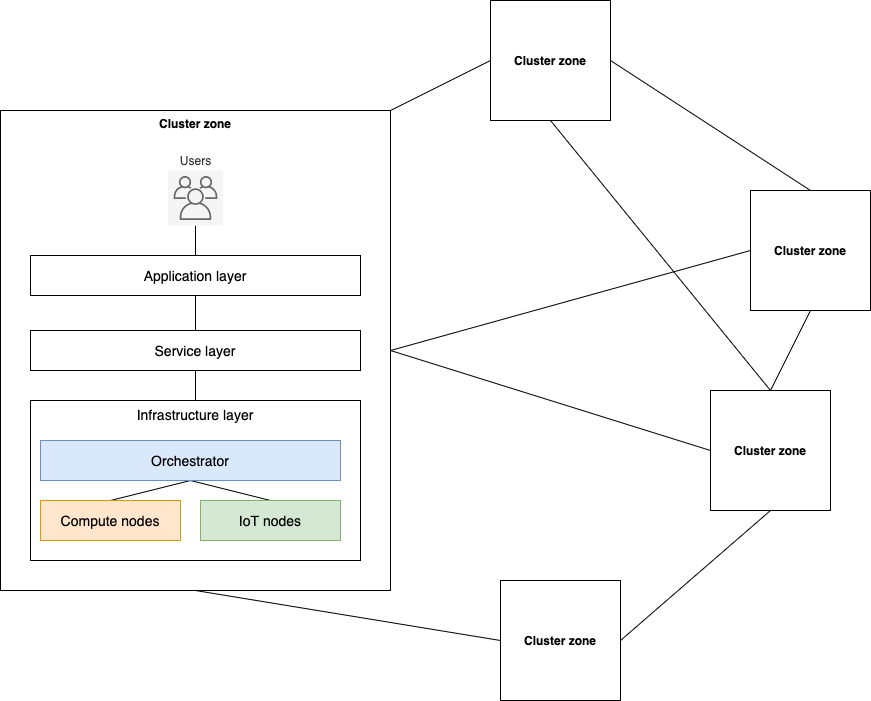
\includegraphics[width=\columnwidth]{figures/architecture-federation}
\caption{A high-level federation architecture \label{fig:architecture-federation}}
\end{figure}

Fig. \ref{fig:architecture-federation} presents a high-level architecture of the system as a federation of \textit{cluster zones}. The federation is responsible for orchestrating the distributed resources across different geographical zones. The rationale for a federation layer is two-fold.

The first goal is to interconnect services, information and computation resources between different areas to support a broader spectre of applications. The federation discovers and aggregates capabilities and capacities of services deployed throughout the cluster zones that compose the computing continuum, and it makes the decisions that guarantee meeting the end-to-end QoS requirements.

The system dynamically instantiates and schedules services along the path from source to destination based on specified requirements and constraints of each application. For the local services, a single cluster zone may not have the necessary hardware or information to support some consumer requirements but could propagate such requests to the federation. The federation would then contact the cluster zones within an acceptable geographical distance based on the service requirements and provide the available options to meet the applicant needs.

Second, a collaboration between cluster zones is needed to support user mobility across regional areas. The services should follow the consumer movements with the slightest perceivable interruption as possible. Synchronisation and state migration are two important mobility issues addressed at the federation layer.

Within a single cluster, users consume applications that in turn contact an intermediary at the \textit{service layer}. Applications define the service requirements and constraints, namely the type of resource, the expected performance and the pricing, without detailed knowledge of the underlying infrastructure. The \textit{orchestrator} receives the requirements from the intermediary, and it provisions the necessary resources and services according to the application's requirements. Then it assigns the latter to \textit{compute nodes} in the cluster, where they are executed. The compute cluster is an abstraction of interconnected nodes on geographically distant clusters, such as clouds and fog nodes.

Developers submit their applications in the form of a manifest. The manifest describes resources requirements regarding the amount of CPU and memory they will require, for example. Likewise, the manifest contains the needed services as well. Services may range from common dependencies like a database and persistent storage to data sources. The orchestrator will determine if the cluster can meet the constraints. Service requirements allow developers to describe constraints on the services, e.g. latency limits and service plans.

This work will not explore further the federation layer because many considerations would be premature at this stage without the necessary preliminary groundwork from the research and industrial communities. The federation architecture is thus an open research question of future works on the continuum.

On the other hand, to the best of the author's knowledge, this paper is the first to combine the computing continuum's vision with a proposal of a technology baseline for the sub-system within a cluster zone. The soundness of the technology baseline is demonstrated with a Proof of Concept (POC). Notably, the POC's goal is to prove that the technologies can be integrated to support the realisation of the continuum's infrastructure layer and evaluate their maturity for such a goal.

The infrastructure layer is composed of a set of service providers that offer data and computational resources. The data can be generated by various streaming IoT devices (e.g. cameras, smartwatches, and smart infrastructure). The computational resources can be heterogeneous and distributed through the infrastructure, from the cloud to the edges.

An additional novel point of this work is focusing on a general-purpose solution to support a wide range of services. The authors of \cite{balouek2019towards} describe a similar framework to combine heterogeneous resources from the edge to the cloud. However, the system is focused on stream-oriented workflows and real-time distributed data processing.

\subsection{Infrastructure architecture}

\begin{figure}[ht]
\centering
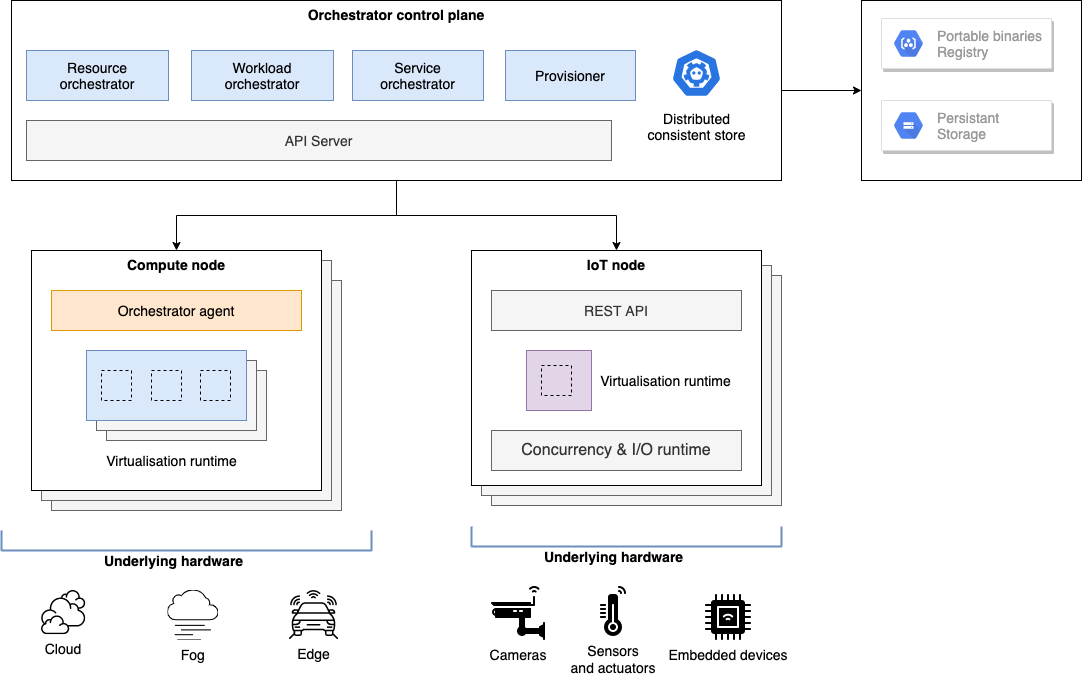
\includegraphics[width=\columnwidth]{figures/architecture-broad}
\caption{Reference architecture for the infrastructure \label{fig:architecture-broad}}
\end{figure}

A reference architecture of the infrastructure is shown in Fig. \ref{fig:architecture-broad}.

\subsubsection{Orchestrator control plane}

The orchestrator control plane is the core of the orchestration system. It has a resource monitor module responsible for keeping track of real-time resource consumption metrics for each node in the compute cluster. The scheduler usually accesses this information to make better optimisation decisions. The scheduler is responsible for determining whether there are enough resources and services available in the continuum to execute the submitted application. If resources are insufficient, applications can be rejected or put on weight until the resources are freed. Another possible solution would be to increase the number of cluster nodes to place the incoming application. Such nodes may be provisioned from local machines or anywhere in the network, typically close to the cluster. After determining if requirements can be satisfied, the scheduler maps application components onto the cluster resources. This deployment is done by considering several factors, e.g. the availabilities, the utilization of the nodes, priorities, or constraints.

In cases where the addition of new cluster nodes is possible, an automatic process is necessary. The provisioner is responsible for dynamically adding nodes (physical or virtual) to the cluster when the existing resources are insufficient to meet the applications' demands. It will also decide when nodes are no longer required in the cluster and shut the nodes down to prevent additional costs.

\subsubsection{Compute nodes}

Each machine in the cluster that is available for services and applications is a compute node. Each of these nodes has an implementation of the orchestrator runtime with various responsibilities. First, it collects local information such as resource consumption metrics that can be periodically reported to the control plane. Second, it starts and stops service instances and manages local resources via a virtualisation runtime. Finally, it monitors the instances deployed on the node, sending periodic status to the control plane.

\subsubsection{IoT nodes}

IoT nodes are embedded devices that act as sensors and actuators, provided as services to the cluster. The IoT nodes are heterogeneous in runtime implementation and communication protocols. Therefore applications in the cluster interface with them via brokers provisioned by the cluster, as explained in Section §\ref{sec:akri}. Besides, the embedded devices support dynamic configuration by running arbitrary virtualisation modules in a lightweight runtime, assuming the module size and the hardware requirements can be satisfied by the limited device.

\subsubsection{Underlying infrastructure}

One of the main benefits of containers is their flexibility in being deployed on a multitude of platforms. Because of these, the cluster machines can be either VMs on public or private cloud infrastructures, physical machines on a cluster, or even mobile or edge devices, among others.

\subsection{Addressed challenges}

This paper attempts to provide some groundwork on how to address the following challenges within the list discussed in Section §\ref{sec:challenges}. For each of the following points, the paper presents a candidate technology that is intended to show a preliminary evaluation of its fitness in the overall system:

\begin{enumerate}
    \item \emph{Service orientation}: the web architecture is proposed as the substrate for the pervasive communication between services in the continuum, and the Representational State Transfer (REST) (§\ref{sec:web}) is the natural architectural style to follow so that services can communicate uniformly. Furthermore, the author presents the Open Service Broker (§\ref{sec:osb}) platform to allow independent vendors and developers to provide services running on popular service orchestrators;
    \item \emph{Orchestration}: Kubernetes (§\ref{sec:kubernetes}) is proposed as an orchestrator for resource orchestration, workload orchestration and service orchestration of the continuum. On this matter, Akri (§\ref{sec:akri}) extends Kubernetes to support the orchestration of IoT devices with an attempt to overcome the heterogeneity and unreliability of the underlying environment;
    \item \emph{Virtualisation}: WebAssembly (§\ref{sec:webassembly}) is used as platform-agnostic virtualisation technology to provide lightweight sandboxing capabilities on every node of the continuum. WebAssembly is a portable bytecode that is a compilation target of potentially any programming language, both the ones that use garbage collection (e.g. Go, JavaScript, and Python) and those that do not (e.g. C, C++, and Rust);
    \item \emph{Dynamic configuration}: the combination of a small WebAssembly interpreter and the low-overhead binary format of the bytecode result in intriguing opportunities for dynamic configuration of IoT devices;
    \item \emph{Interoperability}: REST is a natural choice to support high-level interoperability between services as well. A contribution of this paper is the Rust implementation of the CoAP (§\ref{sec:coap}) protocol to expose constrained devices' capabilities as REST resources. Such resources are then made available within the Kubernetes cluster, easily accessible as RESTful services. Akri's broker-based architecture offers a compelling solution to the heterogeneity of the Internet of Things. Similarly, the Open Service Broker allows a similar opportunity to work around the interoperability issue between cloud providers via a broker-based architecture;
    \item \emph{Portability and Programmability}: the paper suggests using recent efforts in extending and standardising Docker images to support the distribution of arbitrary binary files, notably WebAssembly applications instead of container filesystems. This solution significantly improves the integration with existing development tools and lowers the entry barrier for developing applications in the continuum. The Rust (§\ref{sec:rust}) programming language is then argued as the most sensible choice for providers to implement the infrastructure and developers to realise their applications, especially because of the tight integration to the aforementioned WebAssembly technology;
\end{enumerate}

Due to the ample problem space, mobility, security, privacy, and energy efficiency are not addressed in this paper and are left as open research questions. Besides, by any means, it is also not in the intentions of this paper to be assertive in the technical solutions proposed here. This work intends to present a snapshot of today's technology to evaluate the distance between state of the art and the continuum vision.

Fig. \ref{fig:architecture-technologies} presents the key technologies mentioned above within the reference architecture of the infrastructure.

\begin{figure}[ht]
\centering
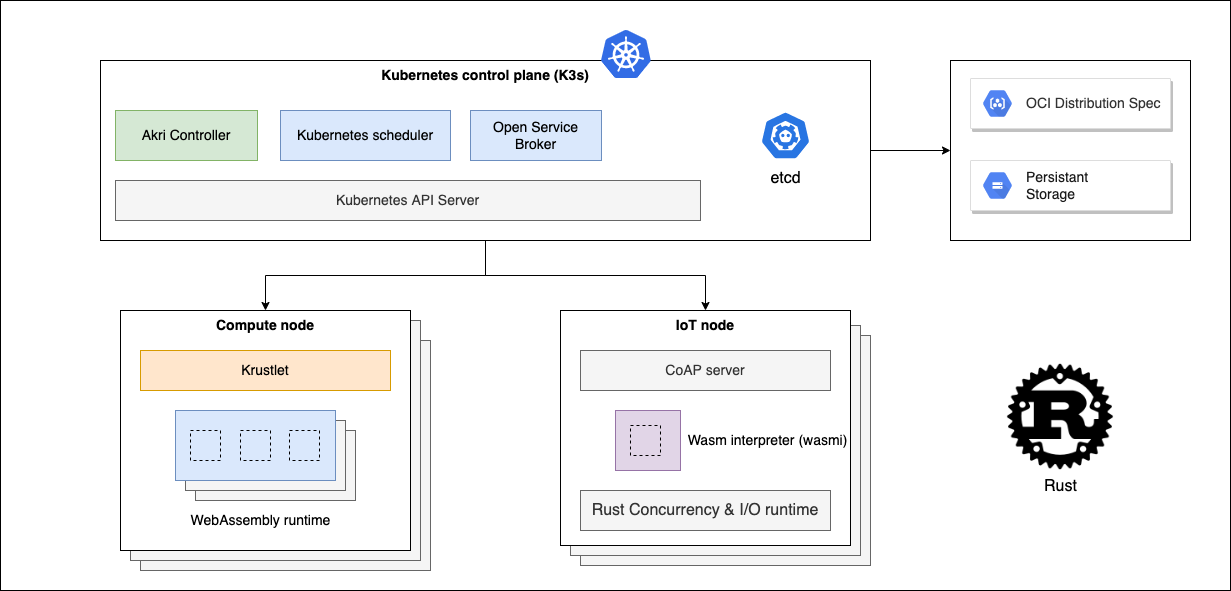
\includegraphics[width=\columnwidth]{figures/architecture-technologies}
\caption{Technology baseline for the reference infrastructure architecture \label{fig:architecture-technologies}}
\end{figure}

\subsection{Web services}
\label{sec:web}

Tim Berners-Lee's original vision for the web focused on documents and their inter-relationships, but it has become more and more a web of applications in the last decade. Nowadays, the web has become the world's most successful vendor-independent application platform.

The web is a loosely coupled architecture and applications today depend on the web architecture, using HTTP to access information and perform updates. The most dominant architectural style is Representational State Transfer (REST) \cite{rest} that makes information available as resources identified by URIs. Applications communicate by exchanging representations of these resources using a transfer protocol, HTTP, precisely. HTTP is the most popular application protocol on the Internet and the pillar of web architecture. However, new communication protocols (e.g. CoAP in Section \ref{sec:coap}) are emerging to extend the web to the Internet of Things and HTTP itself is undergoing revisions (e.g. HTTP/3 or QUIC \cite{langley2017quic}).

The most prominent characteristics of REST that makes it relevant as technology to enabling the continuum are:

\begin{itemize}
    \item Resource orientation: resources are an information abstraction that allows servers to make any information or service available, identified via Uniform Resource Identifiers (URIs). The REST architecture allows the server to own the original state of a resource, and the client negotiates and accesses a representation of it. The representation negotiation is suitable for interoperability, caching, proxying, and redirecting requests and responses. Such features enable seamless interoperation of services in the continuum through proxies, scalable architectures and better availability. Besides, under the REST architecture, web resources often advertise links to other resources creating a distributed web and resulting in an even more scalable and flexible architecture;
    \item Uniform interface: clients access these server-controlled resources in a request-response fashion using a small uniform set of methods with different semantics (GET, PUT, POST, and DELETE). This well-defined, limited set of methods makes REST significantly different from Remote Produce Calls (RPC). The requests are directed to resources using a generic interface with standard semantics that intermediaries can interpret. The result is an application that allows for layers of transformation and indirection independent of the information origin. Such characteristic has been fundamental for the Internet-scale, multi-domain, scalable information system called web. It will be increasingly necessary as the latter expands its scope to the continuum computing. RPC mechanisms, in contrast, are defined in terms of language APIs, not network-based applications \cite{rest};
    \item High-level interoperability: besides the representation negotiation, the REST architectural style enables further interoperability between RESTful protocols through proxies or, more generally, intermediaries that behave like a server to a client and play a client with respect to another server. REST intermediaries play well with the assumption that not every device must offer RESTful interfaces directly. In several cases, notably in the Internet of Things, it may not be possible to change the underlying communication protocol. However, intermediaries allow exposing the resources through a RESTful API nevertheless. The interactions behind that RESTful interface are invisible and may include highly specialized protocols for the specific implementation scenario (e.g. OPC UA or MQTT) \cite{guinard2010resource};
    \item Communication protocol independence: HTTP is a powerful and well-tried protocol. Public APIs benefit from its adoption because it leads to an API accessible from all programming languages and environments without additional technology. On the other hand, HTTP is relatively expensive for both binary overhead and network resource usage. Part of the problem is that HTTP has undergone more than a decade of organic growth, leading to considerable implementation baggage that overwhelms small devices \cite{bormann2012coap}. Fortunately, the REST architectural style is not strictly tied to HTTP, and new communication protocols like CoAP (§\ref{sec:coap}) can offer a very similar interface while guaranteeing more lightweight implementation, less demand for network bandwidth, lower latency and more energy efficiency among many features;
    \item Machine-to-Machine communication (M2M): communication protocols must be specifically designed for efficient M2M communications without introducing overhead in network load, delay, and data processing. In the M2M environments typical of IoT applications (and of the continuum by extension), devices must discover each other and their resources. Resource discovery is common on the web. One form of web discovery occurs when a user access a server's default resource (such as \emph{index.html}), which often includes links to other web resources available on that or related servers. Machines can also perform web discovery if standardized interfaces and resource descriptions are available. New approaches from the IETF include the well-known resource path \emph{/.well-known/scheme} (RFC 5785) and the HTTP link header (RFC 5988). In the IoT, we are dealing with autonomous devices and embedded systems. Therefore the importance of uniform, interoperable resource discovery is much greater than on the current web;
    \item Stateless: REST requires requests from clients to be self-contained, in the sense that all information to serve the request must be part of the request. Statelessness helps applications to scale, as persisting state in a highly distributed system brings challenges like consistency and hinders support for user mobility in the continuum space.
\end{itemize}

From the previous points, it is clear that the design goals of RESTful web systems and the benefits for a decentralized and massive-scale service system align well with the field of pervasive computing. For these reasons, REST an ideal candidate to build a universal API for services and devices in the continuum, letting developers reuse their existing skills and tools. 

\subsection{Open Service Broker}
\label{sec:osb}

\begin{figure}[ht]
\centering
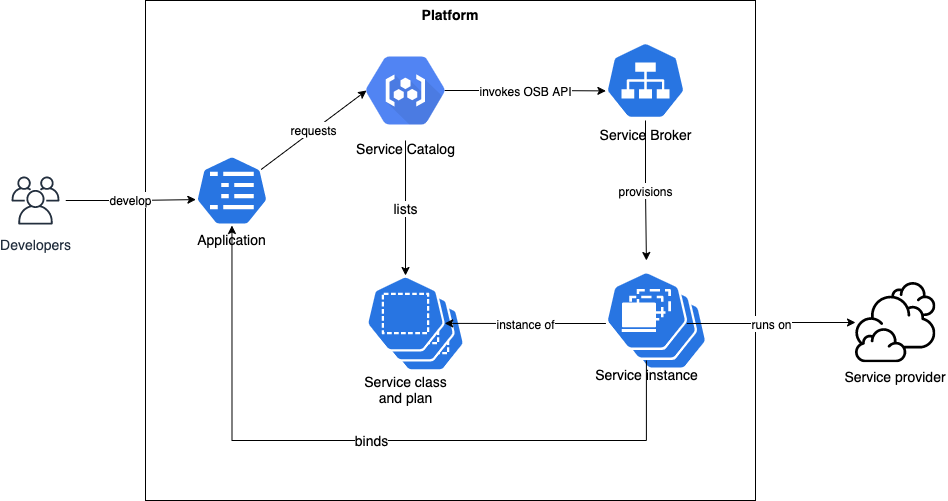
\includegraphics[width=\columnwidth]{figures/osb}
\caption{The Open Service Broker architecture \label{fig:osb}}
\end{figure}

Application developers require services. Managed services, whose infrastructure is handled by a vendor for the whole service lifecycle, enable developers to concentrate on their application code rather than operating these services. On this matter, on-demand marketplace services can increase developer velocity and minimise time to deliver value to the market. In the author's view, the continuum will benefit from a marketplace where vendors develop and add services based on user demand. This idea is not novel, and the most notable example is Cloud Foundry's Marketplace \cite{cloud-foundry-marketplace}, now dismissed, unfortunately. A very akin one, still active and thriving, is the Shopify App Store \cite{shopify} where developers can extend their e-commerce with third-party services. In the continuum's marketplace, providers control the access to the services and payment plans but allow developers to bring their own services to the catalogue. Over the years, a rich ecosystem of services will be developed and accessible via simple well-documented APIs (namely RESTful interfaces).

Contrary to this vision, cloud standards have failed to gain traction. Therefore, the need to find mechanisms for bridging the heterogeneity gap between platforms and enabling data integration is more relevant than ever. Most orchestration technologies working across administrative domains use a broker to orchestrate resources at different levels within a provider (e.g. the cloud and the edge network) and across providers \cite{grozev2014inter}. As the number of cloud vendors is limited, building adapter and brokering layers that align access to different clouds is possible. 

On this matter, several stakeholders (namely the Kubernetes community, OpenShift, IBM and Google) have shown interest and contributed to working on a standard Open Service Broker (OSB) API \cite{osb}. Components that implement the OSB REST endpoints are referred to as service brokers and can be hosted anywhere the application platform can reach them. Service brokers offer a catalogue of services, payment plans and user-facing metadata. The main components of the OSB architecture are presented in Fig. \ref{fig:osb}.

However, the actual value of the broker API is in abstracting service-specific lifecycle operations from the platform. The service broker translates RESTful requests from the platform to service-specific operations such as creating, updating, deletion, and generating credentials to access the provisioned services from applications. Service brokers can offer as many services and plans as desired. Multiple service brokers can be registered with the marketplace so that the final catalogue of services is the aggregate of all services. The platform is thus able to provide a consistent developer experience for application developers consuming these services.

\subsection{Kubernetes}
\label{sec:kubernetes}

\begin{figure}[ht]
\centering
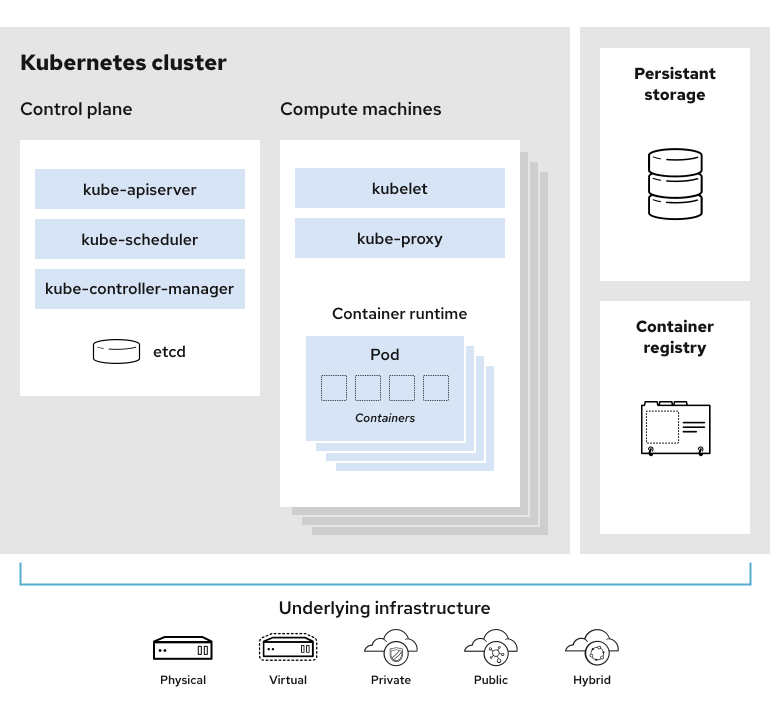
\includegraphics[width=\columnwidth]{figures/kubernetes}
\caption{The Kubernetes architecture \label{fig:kubernetes}. Source \cite{k8s-architecture}.}
\end{figure}

Kubernetes \cite{kubernetes} is an open-source framework designed to manage containerized workloads on clusters and originated from Google's experience with cloud services. Fig. \ref{fig:kubernetes} illustrates the main components of the architecture.

% The basic building block in Kubernetes is a Pod. A Pod encapsulates one or more tightly coupled containers that are colocated and share the same set of resources. Pods also encapsulate storage resources, a network IP, and a set of options that govern how the Pod's container(s) should run. A Pod is designed to run a single instance of an application enabling horizontal scaling by replicating multiple Pods across the nodes. The amount of CPU, memory, and ephemeral storage a container needs can be specified when creating a Pod. This information can then be used to make decisions on Pod placement. These compute resources can be specified as both requests and limits.

Kubernetes allows for various container runtimes from a technical perspective, with Docker natively supported by the platform. Thanks to the Container Runtime Interface (CRI) API standardisation, Kubernetes supports other container technologies such as containerd \cite{containerd} or Firecracker and gVisor mentioned before.

% Moreover, etcd \cite{etcd} is an open-source highly available distributed key-value store and a fundamental part in supporting Kubernetes in managing the cluster nodes and jobs. Specifically, etcd is used to store all of the cluster's data and acts as the single source of truth for all of the framework's components.

Overall, Kubernetes is a highly mature system; it stemmed from 10 years of experience at Google. It is the leading container-based cluster management system with an extensive community-driven support and development base. It provides users with a wide range of options for managing their Pods and how they are scheduled, even allowing for pluggable customised schedulers to be easily integrated into the system.

Besides the extensible scheduler, which makes Kubernetes already an intriguing choice as a potential orchestrator for the continuum, it also supports label-based constraints for the Pods' deployment. Developers can define their labels to specify identifying attributes of objects that are meaningful and relevant to them but that do not reflect the characteristics or semantics of the system directly. An example would allow specifying that an IoT device component must be reachable from the host or persistent storage available, e.g. a Solid State Drive. Nevertheless, more importantly, labels can be used to force the scheduler to colocate services that communicate a lot into the same availability zone, improving the latency drastically and paving the way for context-aware services. % However, to realize the heterogeneity goals, it is required to filter unqualified resources continuously. New resource affinity models should be proposed to rank the resources when provisioning for different applications. 

On the other hand, this work has not explored standard application manifests to describe the service requirements. The POC merely leverages the Kubernetes YAML format, which specifies information like the container image, the placement constraints, and the resource requests.

Finally, Kubernetes is also designed with multitenancy in mind, compared to Docker Swarm \cite{docker-swarm}. Docker Swarm is another popular open-source orchestrator often cited as the main competitor for edge orchestration due to its simplicity (e.g. \cite{bellavista2017feasibility}, and \cite{ismail2015evaluation}). Support for multitenancy is a must and well-aligned with their goal of executing heterogeneous services on a set of shared resources.

\subsubsection{Akri}
\label{sec:akri}

\begin{figure}[ht]
\centering
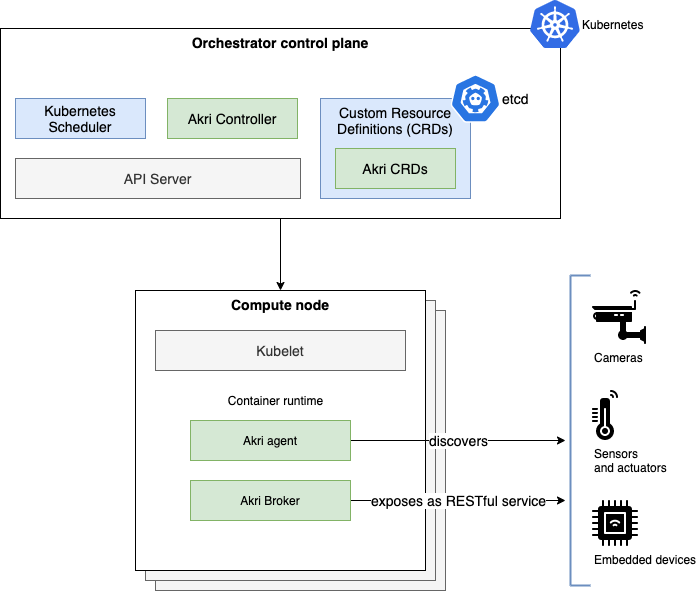
\includegraphics[width=\columnwidth]{figures/akri}
\caption{The Akri architecture \label{fig:akri}}
\end{figure}

Akri \cite{akri} is an open-source project which extends the Kubernetes Device Plugins API \cite{k8s-device-plugins} to allow visibility to IoT devices from applications running within the cluster. The Device Plugin API is designed initially to expose hardware resources attached to a Kubelet, such as GPUs or Solid State Drives, and it is still at the experimental stage. Akri stretched the design further so that it would be possible to implement the discovery of IoT devices, with support for the diversity of communication protocols and the ephemeral availabilities.

Akri's architecture, presented in Fig. \ref{fig:akri}, can be divided into four main components: the agents, the controller, the brokers and the configuration. A configuration is a Kubernetes Custom Resource Definition (CRD) to extend the Kubernetes API with new types of resources. Specifically, a configuration defines a communication protocol (e.g. OPC UA \cite{gruner2016restful}) and the related metadata, such as the protocol discovery parameters or the Docker image to use as agent.

The Akri agent is a Pod responsible for discovering devices according to a communication protocol. It can be easily developed and deployed to the cluster to support new protocols in the system. The agent will track the state of the device and keep the Akri controller updated with the status. At the time of writing, the project has built-in support for ONVIF \cite{onvif}, udev \cite{udev} and OCP UA \cite{gruner2016restful} discovery handlers, with an incoming proposal for CoAP \cite{bormann2012coap} written by this paper's author.

Using Akri, the Kubernetes cluster can carry out dynamic discovery to use new resources as they become available and move away from decommissioned/failed resources. Discovering IoT devices is usually accomplished by scanning all connected communication interfaces and enlisting all locally available resources.

Lastly, the Akri controller advertises discovered leaf devices to the Kubernetes resources manager, making them visible to any application that requires IoT devices to work. The controller is also responsible for enabling applications to communicate with the device and deploying a broker Pod as intermediary. 

The broker is any application instructed to communicate with the device, but Akri does not put constraints on its implementation or programming language. For example, Akri could be configured to deploy a broker that exposes a gRPC \cite{gRPC} interface and translate the requests to the underlying IoT communication protocol. In this paper's view, the broker should be a web server that abstracts the actual communication between devices and applications behind a RESTful API. Such perspective is in line with the reasons presented before to choose the REST architecture as a uniform interface for services in the continuum. Akri should automatically find all the devices in the environment and make them available as web resources. As an instance, the agent discovers the devices regularly by scanning for CoAP (Section §\ref{sec:coap}) resources.

Besides, the broker could offer local aggregates of device-level services. For example, it can offer a service that returns the combined temperature measurements of all the things connected to it at any given time.

A RESTful broker can also help scale with the number of concurrent HTTP requests by implementing highly performant cache mechanisms. The IoT resource periodically sends its sensor readings to the broker, where the values are cached locally. Each application request is then served directly from this cache without accessing the actual device, improving the average roundtrip time.

The broker architecture has the advantage of fully decoupling the leaf node from the cluster workload. It only needs to send an update packet with a frequency short enough to ensure data validity. On the other hand, the retrieved data's staleness will depend on the device's frequency of updates. Forwarding the HTTP request (adequately translated) has the advantage of always returning the most recent sensor reading when the request is processed. The cache mechanism cannot be applied for non-cacheable requests (e.g. HTTP POST) that must be sent to devices, such as turning on LEDs or changing the application state.

As many distributed monitoring applications are usually read-only during their operation (e.g. sensors collecting data), this architecture exhibits a greater scalability level. A potential goal is to enable new types of services where physical sensors can be shared with thousands of users with little impact on latency and data staleness. A representative of such a case is tracking public transportation with sub-second accuracy \cite{elbamby2019wireless}.

\subsection{CoAP}
\label{sec:coap}

\begin{figure}[ht]
\centering
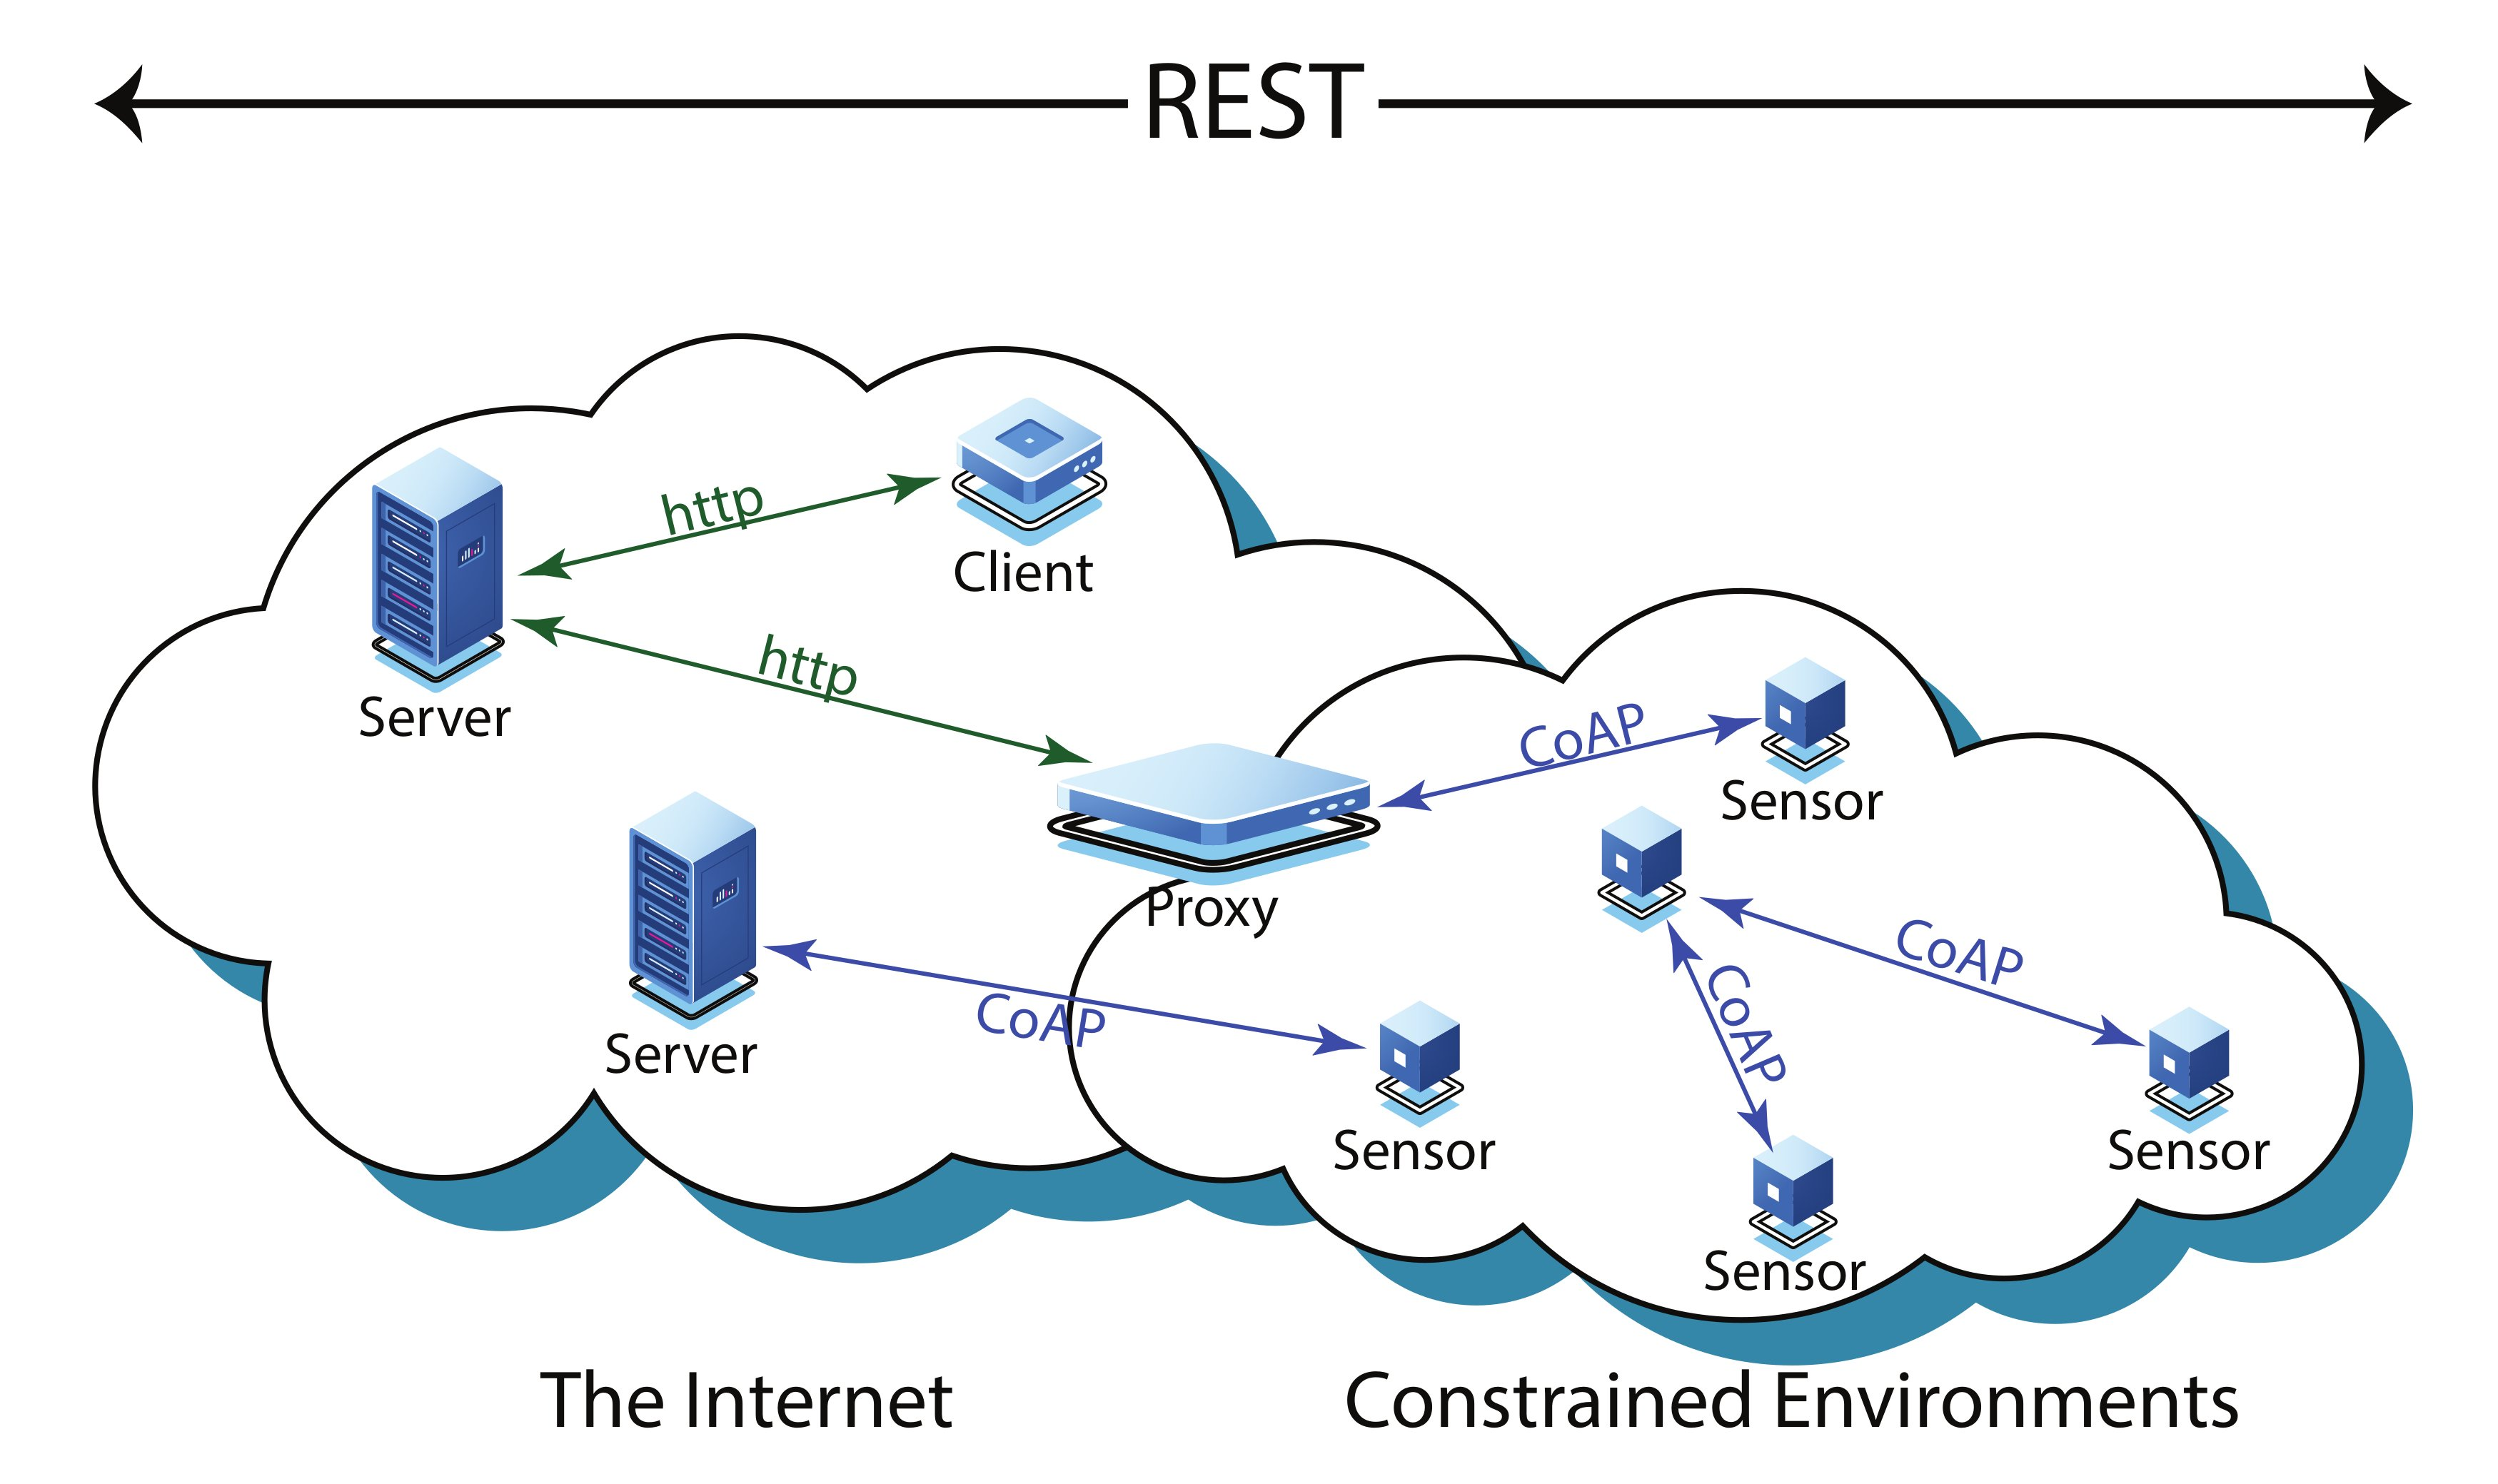
\includegraphics[width=\columnwidth]{figures/coap}
\caption{The REST architecture enhanced with CoAP \label{fig:coap}. Source \cite{bormann2012coap}.}
\end{figure}

CoAP \cite{bormann2012coap} (RFC 7252) is a web communication protocol for use with constrained nodes and constrained (e.g. low-power, lossy) networks. The protocol is designed for M2M applications and provides a client-server architecture between IoT nodes but supports built-in discovery of resources.

A central element of CoAP's reduced complexity is that it uses the UDP transport protocol instead of TCP and defines a very simple message layer for retransmitting lost packets. The rationale for UDP is that TCP carries significant overhead and can have suboptimal performance for links with high packet loss, both of which are common across the Internet \cite{nygren2010akamai} and especially on remote locations where sensors might be deployed. Besides, the HTTP protocol adds further burden, as the additionally multiple round trips required for the requests can quickly add up, affecting the device performance and energy efficiency.

CoAP uses a four-byte binary header within UDP packets, followed by a sequence of options, each up to two bytes. The protocol's specification also defines the usual four request methods: GET, PUT, POST, and DELETE. Similarly, response codes are patterned after the HTTP response codes.

The protocol is built upon key concepts of the web such as URIs and RESTful interaction \cite{pereira2013enabling}. As a result, CoAP easily interfaces with HTTP for integration with web services while meeting specialized IoT requirements such as multicast support, very low overhead and simplicity for constrained environments. 

The URI format allows exposing device data as resources and the use of standard and specialized service endpoints. For instance, CoAP servers are encouraged to provide resource descriptions via the well-known URI \emph{/.well-known/core} to achieve resource discovery. Clients then access this description with a GET request on that URI, usually via an IPv4 or IPv6 broadcast message. The description format is based on the CoRE Link Format (RFC 6690), which is simple and easy to parse. Ease of parsing allows more efficient M2M discovery and inter-communication between the nodes themselves.

% The CoAP protocol supports different resource representations, in line with the REST architecture's representation negotiation. The default format is textual for its convenience when reading and parsing. The binary format is efficient to communicate but requires external tools to make it readable by human users. XML is understandable and very well structured, but the size of its messages is significant, and it is much worse to parse than binary formats. Lastly, JSON is understandable, well structured and compact, but may still put an unnecessary parsing burden on the limited device. With all constrained devices, flash or memory consumption is one of the biggest problems, notably on devices where network connectivity already claims significant buffer memory.

Another advantage of CoAP is that human interactions follow a familiar and intuitive pattern already used by many developers by using standard web technologies. Thus, the learning curve is smoother. This feature cannot be underestimated as allowing developers to use a familiar and seamless programming experience is essential to achieve the continuum's success.

Interoperability with the rest of the continuum can be achieved by following the REST architecture's proxy pattern, as depicted in Fig. \ref{fig:coap}. We can generally build intermediaries that speak CoAP on one side and HTTP on the other without encoding specific application knowledge. This flexibility allows deploying new applications without having to upgrade the intermediaries involved. On the other hand, an intermediary can perform the translation between CoAP and HTTP without posing further requirements either on the client or server. Because equivalent methods, response codes, and options are present in HTTP and CoAP protocols, the mapping between the two is straightforward. As a result, an intermediary (e.g. an Akri broker) can discover CoAP resources and make them available at regular HTTP URIs, enabling web services to access CoAP servers transparently.

However, the HTTP client-initiated interaction model may be unsuited for many event-based and streaming systems in the IoT. Data is sent asynchronously to the clients as soon as it is produced. CoAP uses the Observe approach (RFC 7641) to support pushing information from servers to clients to overcome this issue. A client can indicate its interest in further updates from a resource by specifying the "Observe" option in a GET request. If the server accepts this option, the client becomes an observer of this resource and receives an asynchronous notification message each time it changes. This kind of communication, combined with an intermediary broker, allows streaming data updates via WebSocket (RFC 6455) and overcoming the client-pull interaction model of HTTP. The broker can also help achieve more reliable communication by transparently changing the underlying sensor in case of unavailability or by avoiding closing the connection in case of temporary loss of connectivity.

\subsection{WebAssembly}
\label{sec:webassembly}

\begin{figure}[ht]
\centering
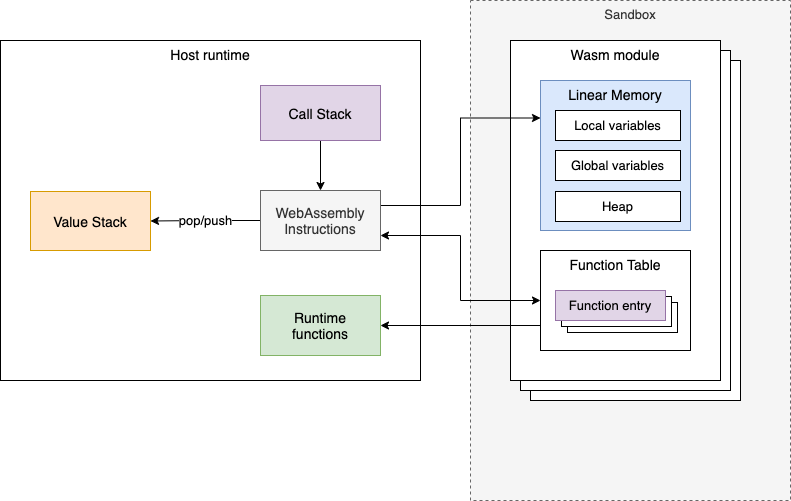
\includegraphics[width=\columnwidth]{figures/webassembly}
\caption{WebAssembly stack machine \label{fig:webassembly}.}
\end{figure}

WebAssembly (Wasm) \cite{haas2017bringing}, first announced in 2015 and released as a Minimum Viable Product in 2017, is a nascent technology that provides strong memory isolation (through sandboxing) at near-native performance with a much smaller memory footprint. WebAssembly is a language designed to address safe, fast, portable low-level code on the web. The project is developed by the World Wide Web Consortium (W3C) with support from all major web browser vendors (Mozilla, Google, Microsoft, and Apple), thus increasing the likelihood that it will avoid serving the purposes of a single entity (e.g. Java and .NET). Developers who wish to leverage WebAssembly may write their code in a higher-level (compared to bytecode) language such as C++ or Rust and compile it into a portable binary that runs on a stack-based virtual machine. Even though WebAssembly technically is a binary code format, it can be presented as a language with syntax and structure. This design choice was intentional since it makes it easier to explain and understand without compromising compactness or decoding ease.

% A Wasm binary takes the form of one or more modules. It contains definitions for functions, globals, tables, and memories. 

The computation is based on a stack machine represented in Fig. \ref{fig:webassembly}: code for a function consists of instructions that manipulate values on an implicit operand stack, popping argument values and pushing result values. However, WebAssembly represents control flow differently from most stack machines. It does not offer simple jumps but instead provides Structured Control Flow (SCF) constructs more akin to a programming language. This design ensures by construction that control flow cannot contain arbitrary branches. The SCF allows WebAssembly code to be validated and compiled in a single pass as well. SCF can also be disassembled to a WebAssembly text format (.wat) that is easier to read and often overlooked but crucial human factor on the web.

A WebAssembly program's memory is a large array of bytes referred to as a linear memory or simply memory. All memory access is dynamically checked against the memory size, and out of bounds access results in a trap. Linear memory is disjoint from code space, the execution stack, and the engine's data structures. Each Wasm memory access addresses linear memory at an offset from the base, $n$, of the linear memory. Thus, some address virtualisation as an address $b$ in the sandbox is located at $b + n$ in physical memory. The Wasm runtime is responsible for translating linear memory accesses and bounds-checking them to prevent accesses outside the sandbox.

Therefore, compiled programs cannot corrupt their execution environment, jump to arbitrary locations, or perform other undefined behaviour, especially when the original language is memory-safe (e.g. Rust §\ref{sec:rust}). At worst, a WebAssembly is subject to exploits regarding data in its memory.

This memory and state encapsulation are applied at the module level rather than at the application level, meaning that a module's memory and functions cannot leak information unless explicitly exported/returned. This granularity in sandboxing is extremely important as security incidents have increasingly exploited vulnerabilities in the dependency chain. Reuse of third-party software is pervasive in modern languages like JavaScript, Rust or Go. As an example, JavaScript (and consequently TypeScript \cite{typescript}) strongly relies on its package manager NPM and the latter has been increasingly subject to security incidents in recent years \cite{npm-security}.

The granular memory encapsulation means that even untrusted modules can be safely executed in the same address space as other code. Additionally, it allows a WebAssembly engine to be embedded into any other language runtime without violating memory safety and enabling programs with many independent instances to exist in the same process. These sandboxing features make WebAssembly a compelling technology upon which to implement a virtualisation stack for the continuum. On the web, the substrate of the continuum, code is fetched from untrusted sources, and it is vital that it can be safely executed on a plethora of language runtimes.

% Another critical safety feature of Wasm is the type system. Code must be validated before it can be executed safely. Validation rules for WebAssembly are defined succinctly as a type system. This type system is, by design, simple. It is designed to be efficiently checkable in a single linear pass to allow parallelisable binary decoding and compilation.
% Moreover, function pointers cannot be dereferenced directly. A call to a function pointer is translated into a function in a runtime table of valid entry points and types. The type of the function is checked dynamically against the expected type in the said entry. The dynamic signature check protects the integrity of the execution environment. In case of a type mismatch or an out of bounds table access, a trap occurs.

With that being said, the design goals of WebAssembly strongly advocate for its suitability for this paper:

\begin{itemize}
    \item \emph{Safe to execute}: protection for arbitrary code has traditionally been achieved by providing a managed language runtime that enforces memory safety, preventing programs from compromising user data or system state. However, managed language runtimes have traditionally not offered much for portable low-level code, such as C/C++ applications, that do not need garbage collection;
    \item \emph{Fast to execute}: low-level code like that emitted by a C/C++ compiler is typically optimized ahead-of-time. On the contrary, managed runtimes and sandboxing techniques have typically imposed a steep performance overhead on low-level code. WebAssembly is, however, very competitive with native code, and benchmarks using Wasm runtimes on modern browsers have shown a slowdown of approximately 10\% compared to native execution and almost always within 2x \cite{haas2017bringing};
    \item \emph{Language, hardware, and platform independency}: as mentioned before, the web spans not only many device classes but different machine architectures, operating systems, and browsers. Code targeting the web must therefore be independent of any underlying hardware or platform to allow applications to run across all software and hardware types with the same behaviour;
    % \item \emph{Deterministic and easy to reason about}: WebAssembly has been designed with formal semantics from the start for both execution and validation. Besides, the Wasm binary can be compiled into a .wat file to simplify learning and debugging;
    \item \emph{Simple interoperability}: WebAssembly is similar to a virtual ISA in that it does not define how programs are loaded into the execution engine or how they perform I/O. The embedder (i.e. the host runtime) defines how modules are loaded, how imports and exports between modules are resolved, provides foreign functions to accomplish I/O, and specifies how traps are handled. It is possible, by design, to link multiple modules that different authors have created from likewise different source languages. However, as a low-level language, WebAssembly does not provide any built-in object model. It is up to developers to map their data types to numbers or memory. This design is supposed to provide maximum flexibility to developers, and unlike previous VMs like Java or .NET, it does not privilege any specific programming or object model while penalizing others. The downside of this design is that interoperability with object references is cumbersome. It involves exchanging references between the Wasm application and the host code or between modules that originated from different languages. A step in easing this issue is the recent introduction of Reference Types \cite{reference-types}. On the other hand, since WebAssembly is an abstraction over hardware, not over a programming language, a WebAssembly module may be compiled once and moved freely between different hardware architectures with no recompilation;
    \item \emph{Compact}: the binary code is designed to be compact, especially compared to bytecode in text format. For this reason, it is recommended to distribute the binary code on the Internet and use the text format only for learning and debugging. Code transmitted over the network has to be as compact as possible to reduce load times, save potentially expensive bandwidth, reduce memory usage on constrained network-attached devices and improve overall responsiveness;
    % \item \emph{Easy to validate and compile}: validation proceeds by checking on the fly while the incoming bytecodes arrive, with no intermediate representation (IR) being constructed. Benchmarks run on mainstream browsers in \cite{haas2017bringing} prove that validation can be fast enough to be performed at a full network speed of 1Gib/s;
    \item \emph{Streamable and parallelisable}: a Wasm runtime can minimise latency by starting streaming compilation as soon as function bodies arrive over the network. It can also parallelize the compilation of consecutive function bodies. For instance, each function body is preceded by its size so that a decoder can skip ahead and parallelize even its decoding. Minimising the latency is essential for increased mobility, quick release of resources, and support for low-latency use cases.
\end{itemize}

Despite the name WebAssembly, there has been a significant effort in the last years in adopting Wasm for native execution, as it is a portable target for the compilation of various high-level languages. Wasm standard does not necessarily make browser-specific assumptions, and there has been substantial work to standardize the WebAssembly System Interface (WASI) to run Wasm outside the browser. To the best of the author's knowledge, the original design goals assumed a browser-based execution context. Nevertheless, such goals fit perfectly to the continuum's needs, where the web is the infrastructure upon which applications and services are deployed. On this matter, browsers are very much akin to an Operative System for client web applications, and WebAssembly is thus unsurprisingly being adopted on conventional OSes as well. Native execution and browser execution share many problems, like isolation, portability and interoperability, to name just a few.

\begin{figure}[ht]
\centering
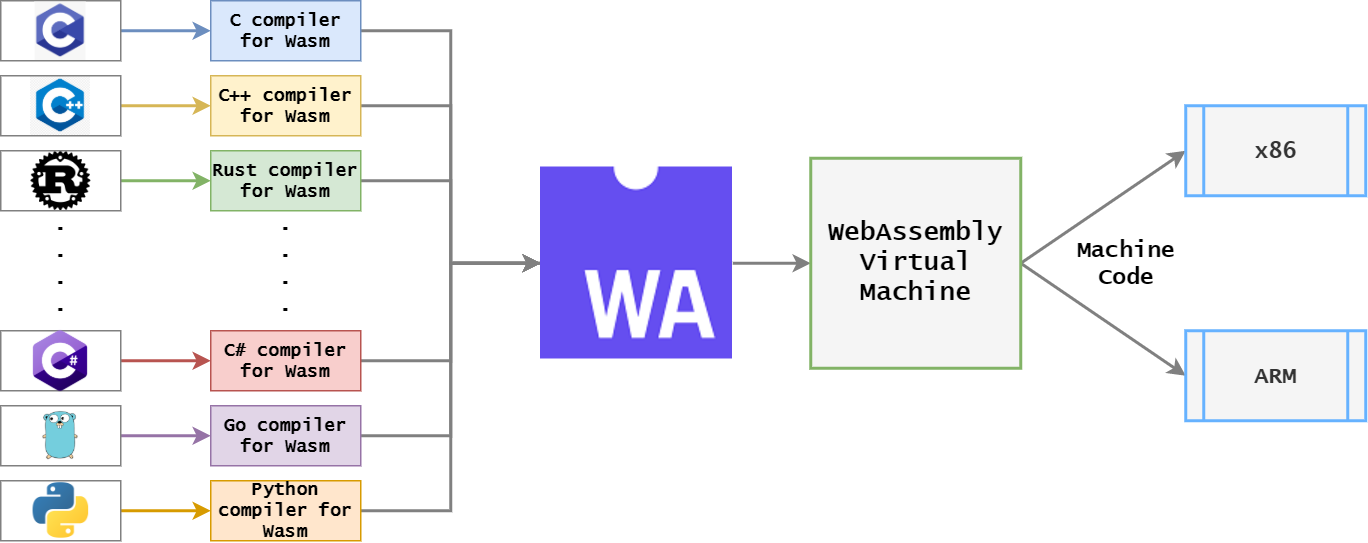
\includegraphics[width=\columnwidth]{figures/portability}
\caption{WebAssembly is a portable binary format \label{fig:portability}.}
\end{figure}

At the time of writing, there are several Wasm runtimes for programs written in different languages capable of embedding Wasm applications. On the other hand, multiple compilers can compile languages to Wasm, as shown in Fig. \ref{fig:portability}. Notably, the Wasm back-end for LLVM \cite{llvm} works for C, C++, and Rust. Commercial solutions have also been slowly but steadily gaining popularity. Cloudflare's Service Workers \cite{cloudflare-workers} began to offer support for creating and hosting serverless functions in WebAssembly. In March 2019, the edge-computing platform Fastly had announced an open-sourced Lucet \cite{fastly-lucet} that provides a compiler and runtime to enable native execution of Wasm applications and can instantiate a Wasm module within $50\mu s$, with just a few kilobytes of memory overhead. Parity is also actively experimenting with writing smart contracts using Wasm \cite{parity-wasm}.

WebAssembly is currently under experimentation as a new method for running portable applications without containers because of its design features. This method leverages its binary format as a portable vehicle to inherent memory and execution safety guarantees via its language features and a runtime with strong sandboxing capabilities. The Wasm security model enables the execution of multiple untrusted modules in the same process, thereby providing significantly more lightweight isolation compared to VMs and containers for multi-tenant serverless execution \cite{gadepalli2020sledge}.

This idea is still in its infancy, but there has been some interest in recent years, as shown by the works done in \cite{hall2019execution} and \cite{shillaker2020faasm}. All these works focus primarily on serverless computing via WebAssembly, demonstrating the popularity of such a computing model. As this paper has stated before, however, if serverless were the only execution model, it would severely limit the variety of applications in the continuum.

\subsubsection{WebAssembly for embedded microcontrollers}

An emerging use case for WebAssembly is arbitrary code execution on microcontrollers, and, as a result, interpreters are gaining popularity on resource-limited devices. wasm3 \cite{wasm3} is a popular open-source interpreter capable of running on any system with at least 64KiB of storage and 10KiB of memory. The authors of eWASM \cite{peach2020ewasm} have also explored various mechanisms for memory bounds checking and have evaluated the trade-offs between processing efficiency and memory consumption. Just-In-Time compilers for WebAssembly exist (e.g. Wasmtime \cite{wasmtime}) and receive more attention from the community, but their size and complexity make them unsuitable for microcontrollers.

Although WebAssembly interpreters can often be approximately 11x slower than native C \cite{wasm3-performance}, they help dynamically update system code and debugging but may not be applicable for code on devices susceptible to performance and energy efficiency.

In the author's view, interpreting WebAssembly on microcontrollers remains an intriguing technology nevertheless worth the research community's attention. They offer a persuasive alternative to other language runtimes, e.g. Lua, which are commonly used on embedded devices to support dynamic configuration \cite{brzoza2016embedded}. The WebAssembly standard has many features that make it appealing for embedded devices \cite{peach2020ewasm}.

\begin{itemize}
    \item Portability: WebAssembly is a platform-independent Intermediate Representation that can be generated from different source languages and can run on many CPU architectures. Solving how to run WebAssembly on microcontrollers effectively would open the possibility to include the embedded world to the continuum as an additional place of intelligent computing, rather than only as a mere data collector and dummy actuator;
    \item Broad support: there is a steadily increasingly ecosystem of vendors, tools, and languages providing WebAssembly support. With the ability to leverage WebAssembly, the embedded system community would benefit from a broader ecosystem;
    \item No mandatory garbage collection: many broadly used language runtimes such as JavaScript, Lua, or python cannot provide predictable execution and may require excessive memory for a microcontroller;
    \item Lightweight runtime: WebAssembly mandates only a small number of runtime features around maintaining memory sandboxing. These light requirements help in an embedded adaptation.
\end{itemize}

\subsubsection{Wasm images}

TODO.

\subsection{Rust}
\label{sec:rust}

As the continuum integrates compute support across the network, the attack surface greatly increases consequently. Security has to be a top priority during software development, yet most of the infrastructure is programmed using the C, C++ programming languages. These two programming languages are chosen due to the low overhead on memory and the high processing performance. Embedded systems have favoured the two languages because of the need for low-level control over the hardware. However, C and C++ are not particularly renowned for producing secure software, as evidenced by the many vulnerabilities reported against the software written in them. Notably, the leading cause of security vulnerabilities are memory safety bugs like data races and buffer overflows. Even higher-level languages suffer from these kinds of safety issues. The Go language, upon which most modern distributed systems are built (namely Kubernetes), is not exempt from exploits based on data races \cite{go-data-races}.

On the other hand, Rust is a strongly-typed, compiled language that uses a lightweight runtime similar to C. Unlike many other modern languages, Rust is an attractive choice for predictable performance because it does not use a garbage collector. It provides strong memory safety guarantees by focusing on "zero-cost abstractions", meaning that safety checks are done at compile-time and runtime checks (e.g. out-of-bounds access) have the minimum overhead and come with a predictable cost.

% Not all operations can be verified to be memory safe at compile time. One example is indexing a slice, a partial view into an array. In this case, the indexing operation contains a runtime check to check if the index is within bounds. If the index is out of bounds, then the result is panic. A panicking condition can either abort the whole program or just unwind the stack of the thread that ran into the panic. The unwinding process walks up the stack freeing all live resources before terminating the thread, ensuring a clean memory state afterwards.

There is a strong emphasis on building safe abstractions with almost zero runtime cost in the Rust community. Safe Rust code is guaranteed to be free of null or dangling pointer dereferences, invalid variable values (e.g. casts are checked), reads from uninitialized memory, unsafe mutations of shared data, and data races, among other misbehaviours.  The borrow checker, the most innovative feature of the language compiler, runs as part of the compilation process and catches bugs like just mentioned misbehaviours. Security cannot be achieved without memory safety, so it is fundamental that the latter is a property of the language and not a developer's concern only.

In the author's view, Rust is a much-recommended choice as the default implementation language for the continuum's infrastructure. Rust is an alternative to C and C++ that can equally compete in performance, low-level control and cross-platform support. Its use cases are not limited to system development, however. Although initially advertised as a system language, Rust is nowadays described as a language to build \emph{any} reliable and performant software. Use cases range from embedded systems and Operative Systems to web servers and user interfaces (e.g. via WebAssembly on the browser). Thanks to its vast community of open-source libraries and productivity tools, it can be a sensible alternative even for high-level services.

Its toolchain is backed by the LLVM modular compiler infrastructure, which Rust relies on for translating high-level code to its LLVM representation (IR). In addition to code translation, LLVM also provides several tools that aid optimisation and dead code elimination. Thanks to the integration of LLVM, the Rust compiler can transform this IR to generate WebAssembly binary code. The union of Rust and WebAssembly constitutes a powerful combination. Developers can write source code in Rust to achieve high productivity and efficient memory-safe applications. On the other hand, WebAssembly can contribute with a hardened execution environment and universally portable binaries. Developers would not need to compile or distribute multiple versions (e.g. Docker image versions) of the same software. 

% \subsubsection{RTIC}

% Rust is gaining popularity as a language for embedded systems as well. The language provides a rich standard library, which relies on dynamic memory allocation provided by the host operating system, not available on embedded devices. Fortunately, the standard library is built on a core library that neither requires dynamic allocations nor any host operating system. These minimal dependencies make it possible for Rust applications to be built and executed on bare metal targets. Likewise, many Rust libraries that may be needed on embedded environments come with support for "no\_std", i.e. the library can be compiled without the standard library. 

% The Rust compiler rustc supports a wide range of platforms and architectures as well. Passing a compilation target to rustc allows compiling the source code to machine code optimized for the target platform.

% A further step towards the maturity of Rust as a language for embedded systems is the framework Real-Time Interrupt-driven Concurrency (RTIC) \cite{rtic}, previously known as Real-Time For the Masses (RTFM) \cite{eriksson2013real}. RTIC is a framework developed by the Embedded Systems group at the Luleå University of Technology (LTU) for leveraging the interrupt controller (shortly explained) to schedule tasks of different priority. At the same time, the risk of deadlock is mitigated thanks to all resource-accesses being handled by the Stack Resource Policy (SRP) \cite{baker1990stack}.

% The Stack Resource Policy is a method to handle resource access in real-time systems with a single shared stack. RTIC uses SRP to handle access to resources, and it guarantees a race and deadlock-free preemptive execution, along with bounded priority inversion. Additionally, the model does not use excessive memory for the stack since all the tasks share a common stack space.

% RTIC implements the SRP using hardware interrupts. An interrupt signal is a hardware-generated event that usually occurs asynchronously with respect to the program's execution. Examples of signals include an electrical pin changing its logical state from 0 to 1 or vice versa, a timer reaching a specific value, or data becoming available on some communication interface. In response to these signals, the processor executes an interrupt handler, a special subroutine. Interrupts also have an associated priority level. In the ARM Cortex-M architecture case, all interrupts have higher priority than the thread mode, reserved for the common procedures, so handlers will preempt code running in thread mode.

% Preemption works as follows: the processor suspends the execution of the current subroutine, saves the state of that subroutine (the processor registers) onto the stack and then jumps to the interrupt handler. The interrupt handler runs to completion and returns. Upon returning from the interrupt handler, the suspended routine's state is restored by popping the registers off the stack, and the preempted routine is resumed.

% The Nested Vector Interrupt Controller (NVIC) manages all these interrupts peripheral \cite{joseph2014definitive}. The NVIC is a standardized interrupt controller found on all Cortex-M devices. The NVIC provides an interface to control and configure interrupts in the form of memory-mapped registers.

% The way the NVIC handles interrupts \cite{interrupts-handling} exactly matches how the RTIC task model prioritizes tasks. This fact is used to provide a highly efficient implementation: the RTIC runtime lets the NVIC, the hardware, do all the task scheduling, so no bookkeeping needs to be done in software. Thus, the task's priority is bound to the interrupt service routine (ISR), matching that priority, associating an ISR to each interrupt handler, represented by a task. This alternative to time-sliced threads provides several advantages like reduced overhead, efficient memory utilization, predictable performance (constant time overhead), deadlock freedom, and suitability for static analysis \cite{eriksson2013real}.

\section{Evaluation}
\label{sec:evaluation}

In this section, the author presents a performance evaluation of the Proof of Concept (POC) that implements the technology baseline presented in Fig. \ref{fig:architecture-technologies}. The evaluation uses a local cluster of 4 machines and a microcontroller constituted by:

\begin{itemize}
    \item 4 Raspberry Pi 4 Model 3B+ with Quad-core Cortex-A53 (ARMv8) 64-bit SoC at 1.4GHz and 1 GB physical memory. The Raspberry 3B+ model has been chosen to showcase the feasibility of the presented technologies on limited low-powered machines, relatively cheap and with only 1GB of memory;
    \item A STM32F407 microcontroller with ARM Cortex-M4 core, 512KiB flash storage, and 128KiB of memory. The device is also capable of many 32-bit floating-point operations.
\end{itemize}

Raspberry Pi and STM32F407 microcontrollers are designed for moderately high computational performance, low unit cost, and power efficiency in edge computing environments. The author believes that this evaluation's results should generalize to other ARM machines and microcontrollers in the Cortex-M family.

On the software layer, the evaluation uses Rust 1.53.0-nightly (07e0e2ec2 2021-03-24) and Alpine Linux aarch64 v3.12.1 as OS for the Raspberry Pi. Alpine Linux has been chosen as it is a much more lightweight alternative to Ubuntu, and it offers a built-in Raspberry Pi version available for download. An idle Ubuntu Server 20.0 consumes about 420MB, whereas Alpine Linux incurs only 50MB of memory.

\subsection{The application}

As a practical example to guide the architecture's implementation, the paper applies the continuum concept to a flood warning system. In a flood warning system, the telemetry stations acquire data from wireless sensors networks, process the data in a distributed manner, and locally determine potential levee breaking. Sensor networks represent a crucial component in IoT environments \cite{yu2017survey}. They are typically composed of a potentially high number of sensing nodes, communicating in a wireless multi-hop fashion. Such networks can provide various valuable data and are being utilised in several areas like healthcare, government and environmental services, defence (military target tracking and surveillance), hazardous environment exploration, and seismic sensing.

The existence of preprocessed data in the local sensor-actuator networks can be leveraged to support timely disaster analysis. On the other hand, the geographical distance between the networks, the volume of data, and the relatively low interest (when no significant event is happening) make a centralised vertical solution undesired \cite{balouek2019towards}. Thus, the distributed architecture of the continuum is proposed as a viable architecture for advanced telemetry systems with distributed intelligence.

The ideas and a large part of the implementation, which the paper applies to the smart levee monitoring system, can also be applied to other modern data acquisition and distributed processing systems with similar requirements, including smart cities and smart agriculture. Risk assessment and early warning systems play a crucial role in minimizing the negative results of floods. Such systems may significantly contribute to detect a potential threat of a breach. Therefore, local flash floods may be dangerous because they occur in a short time, usually as a result of sudden heavy rainfall.

\begin{figure}[ht]
\centering
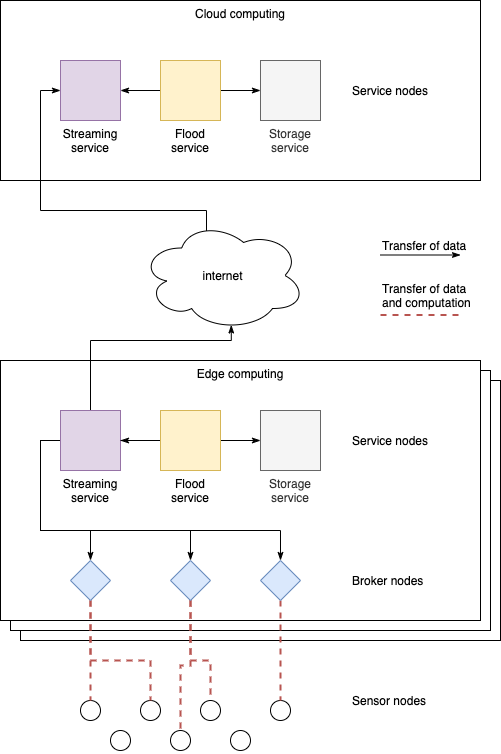
\includegraphics[width=\columnwidth]{figures/architecture-levee2}
\caption{Architecture for the flood warning system \label{fig:architecture-levee}}
\end{figure}

The application implements a system based on the architecture proposed in Fig. §\ref{fig:architecture-levee}:

\begin{itemize}
    \item Sensor nodes: they composed of sensor devices that collect data, preprocess it and transmits it to the edge cluster for further processing. One challenging task of this layer is implementing the dynamic configuration of the internal logic, as preprocessing can result in more accurate predictions, less bandwidth usage and more energy efficiency. The arbitrary code execution is safely enabled by running a WebAssembly interpreter on the Wasm binary file. The portable low-overhead Wasm format unlocks transfer of computation to dynamically instruct the sensor nodes about the preprocessing logic on a case-by-case basis;
    \item Broker nodes: they expose the sensor nodes behind a RESTful interface. At this stage in Akri, each sensor node discovered by Kubernetes has an associated broker responsible for the communication with the rest of the services. However, a single broker should be able to aggregate the data from multiple sources. The broker subscribes to the IoT REST resources via a CoAP message, and the device periodically sends CoAP updates, which are forwarded to the cluster services as WebSocket packets. The broker ensures that both parts, IoT nodes and services nodes, are independent as far as they agree to communicate following the REST architecture. Service nodes typically use REST over HTTP, while sensor nodes prefer CoAP;
    \item Service nodes: they implement the services needed by the flood warning system and allow them to be reused across different clusters. The use case needs a streaming service to aggregate the data from the device brokers, a local database to store the information for the analysis, and a flood prediction service to analyse the information and provide insight. 
\end{itemize}

The service nodes are deployed at multiple edge clusters, corresponding to different stations, and at a cloud cluster. The rationale for expanding the services to the cloud is two-fold.

First, the edge clusters are heterogeneous in computing capacity, and some zones may have not enough computing power to handle streams. Leveraging the cloud can help increase the workload at the cost of more bandwidth usage and latency. Such compromise might be acceptable, especially in the case of intensive data analysis on the sensor data.

Second, the prediction model could benefit from more knowledge derived from multiple streams geographically distributed. Likewise, a flood risk assessment model running in the cloud could achieve a globally optimal solution, whereas edge services can output only locally optimal results. On the other hand, during flood threat scenarios, the communication channels may become unavailable, so the system must perform a localised assessment. Unfortunately, the loss of communication is unpredictable, but the system must quickly adapt to the scenario. Such computing dynamism is a perfect scenario where the continuum shines compared to relatively static cloud-only, edge-only, or pre-defined cloud+edge architectures.

\subsection{Evaluation of WebAssembly for microcontrollers}

\begin{figure}[ht]
\centering
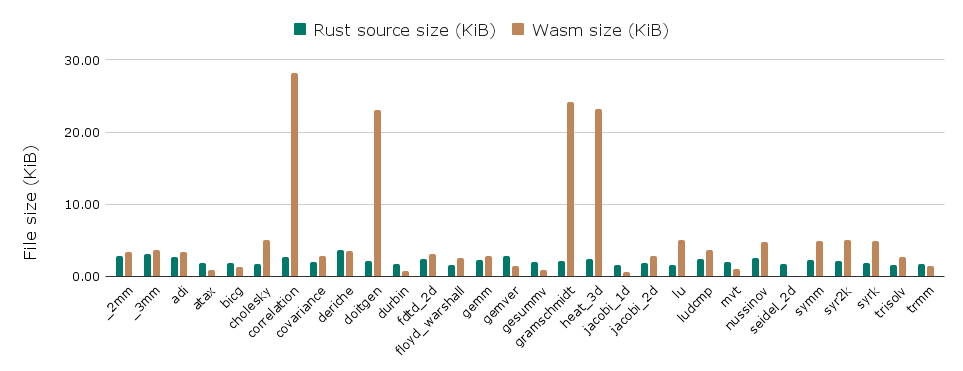
\includegraphics[width=\columnwidth]{figures/b-wasmi-2}
\caption{Comparison of Wasm size (KiB) and Rust source size (KiB) \label{fig:b-wasmi-2}}
\end{figure}

\begin{figure}[ht]
\centering
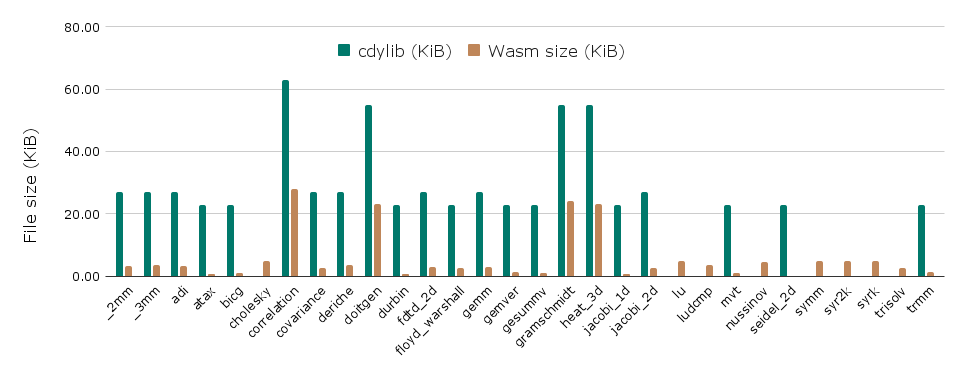
\includegraphics[width=\columnwidth]{figures/b-wasmi-3}
\caption{Comparison of Wasm size (KiB) and C dynamic library size (KiB) \label{fig:b-wasmi-3}}
\end{figure}

Fig. \ref{fig:b-wasmi-2} and Fig. \ref{fig:b-wasmi-3} present a comparison of the sizes of different Wasm binaries compiled from the Polybench \cite{yuki2014understanding} modules. The Polybench benchmark suite offers relevant functions to embedded systems as it includes common matrix and statistical operations.

Fig. \ref{fig:b-wasmi-2} offers a direct comparison of binary size and source size. However, comparing with source code is rarely meaningful due to factors including the widespread use of conditional compilation and unpredictable build behaviours. The purpose is to achieve an initial grasp of the Wasm binary size. The author has attempted to control for these effects by configuring the Rust toolchain to reasonable defaults. The compiler is configured to rely on LLVM to optimize the resulting code for code size. The toolchain also uses LLVM's link-time optimization (LTO) to ensure further size optimisation.

Once the compilation process is done, the result is a self-contained, sandboxed Wasm binary file ready for deployment onto the continuum.

The results show how the final Wasm binary size has no predictable correlation to the source size, despite being usually about 2x larger, with some exceptions. Modules like "correlation" show a significant increase in the Wasm size relative to source code lines. Such a variety of differences depends on the source code's specific instructions and the toolchain configuration. Notably, loops, inlined functions and math functions can result in substantial differences in the output size because of the different optimisation techniques the compiler may take. Such unpredictability means that the Wasm toolchain is not immune to the compilers' famous idiosyncrasy, and developers must be careful always to check the final output.

This work has also chosen the C dynamic library size as a more meaningful comparison since it is a close alternative to Wasm binary files. Both outputs have been compiled using the same LLVM toolchain and optimisation flags. In such a case, the results undeniably favour the Wasm binary format as the C dynamic lib is often many times larger. The author has even removed some of the Polybench modules (namely \emph{cholesky, lu, ludcmp, nussinov, symm, syr2k, syrk, and trisolv}), which had a significantly larger C dynamic library size of 1.5MB (compared to about 5-10KiB in Wasm), which would make the other modules in the chart visually hard to evaluate. Comparing Wasm files to containers would greatly favour the former, as containers package a whole operative system filesystem. Even the smallest image base, "Alpine Linux Mini Root Filesystem", has an additional size of about 5.5MB uncompressed.

\begin{figure}[ht]
\centering
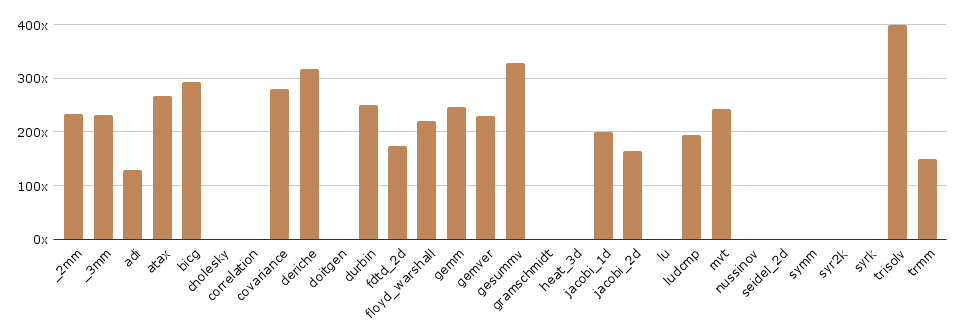
\includegraphics[width=\columnwidth]{figures/b-wasmi-4}
\caption{Comparison of Wasm interpreter performance and Rust native performance \label{fig:b-wasmi-4}}
\end{figure}

Fig. \ref{fig:b-wasmi-4} offers an overview of the Wasm interpreter's execution performance on the STM32F407 microcontroller. Each Polybench benchmark has been run 15 times, following the same methodology described in \cite{wasm3-performance}. The results show a dramatic slowdown compared to the Rust native alternative, with a factor of 100-400 times. Such results are discouraging for the idea of using Wasm interpreters on microcontrollers to support dynamic reconfiguration.

However, it is fair to note that the Wasm interpreter wasmi \cite{wasmi} was adapted to work on embedded devices and was not designed for highly constrained devices. wasmi is developed by Parity, a blockchain company, and is thus used to offer a deterministic sandboxed execution context running on cloud servers. As a result, execution performance is not paramount, unfortunately. The alternative interpreter wasm3, implemented in the C language, shows a much minor execution penalty, in the order of 30-60x slower than native \cite{peach2020ewasm}. Thus, it is reasonable to believe that future efforts may allow a comparable result for the Rust-built wasmi interpreter. Nevertheless, 30x times execution over time can still arguably deter the usage of interpreters in microcontrollers. Future work should also provide a benchmark with respect to other popular interpreted languages like Lua, Python, and JavaScript.

\begin{figure}[ht]
\centering
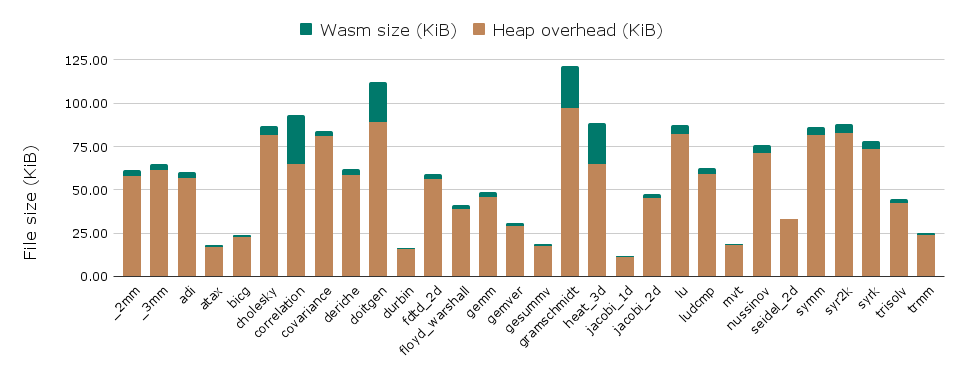
\includegraphics[width=\columnwidth]{figures/b-wasmi-1}
\caption{Comparison of Wasm size (KiB) and heap overhead (KiB) \label{fig:b-wasmi-1}}
\end{figure}

As an additional benchmark, the author has evaluated the heap overhead of interpreting Wasm on microcontrollers. Fig. \ref{fig:b-wasmi-1} presents a significant increase in the heap usage with respect to the Wasm size. However, the most crucial concern is that such a heap increase is not predictable. Such unpredictability does not come in favour of the usage of WebAssembly on microcontrollers, as embedded devices have extremely limited resources and must have predictable behaviours to ensure proper real-time execution. Such deficiency is an intrinsic issue with interpreters, as the code instructions and execution data structures must be stored in heap memory. This behaviour contrasts with the binary executables that can save and access instructions or read-only data on the more capable flash storage. Writable data is saved in the stack instead, and it can be calculated with accuracy in many production-grade toolchains like C and Ada.

Generally speaking, running Wasm on resource-constrained microcontrollers has also presented other challenges.

\begin{itemize}
    \item Memory consumption: Wasm's 64 KiB pages are too large for microcontrollers that often have between 16-256 KiB SRAM. Dynamic allocation is a common requirement even for embedded systems. However, Wasm specifies that the sandbox should expand the memory by 64KiB chunks, which is not granular enough for constrained embedded systems. As a consequence, the wasmi interpreter has been modified to allocate non-standard pages of 16KiB. Otherwise, it would have been impossible to execute any benchmark on the STM32F407 microcontroller, as additional heap space is required for the interpreter's internal structures and the Wasm instructions themselves. There is a need for a Wasm embedded standard that supports smaller granularity of memory pages;
    \item Assumed floating-point operations: Wasm specifically is a 32-bit virtual architecture and supports floating-point, but not all Cortex-Ms do. In such cases, floating-point emulation must be provided by the programmer. In Rust, this solution is typically accomplished utilising the \emph{libm} library, a port of MUSL's libm containing the most popular math operations. MUSL is a lightweight alternative to the conventional libc and employed as an alternative in Alpine Linux. However, the Rust ecosystem is less mature and complete on this matter than the C version, and the many floating-point functions are still missing in libm. 
\end{itemize}

% \subsection{Evaluation of CoAP for microcontrollers}

% \begin{figure}[ht]
% \centering
% 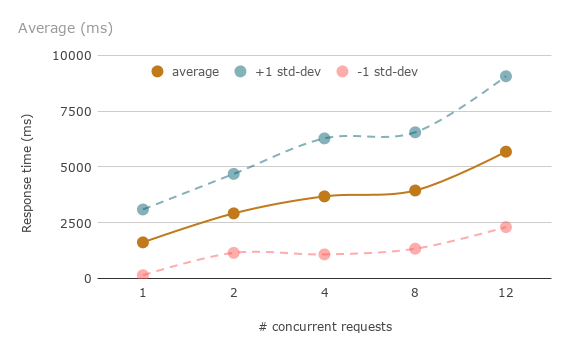
\includegraphics[width=\columnwidth]{figures/b-coap-1}
% \caption{Average response time for concurrent CoAP requests \label{fig:b-coap-1}}
% \end{figure}

% \begin{figure}[ht]
% \centering
% 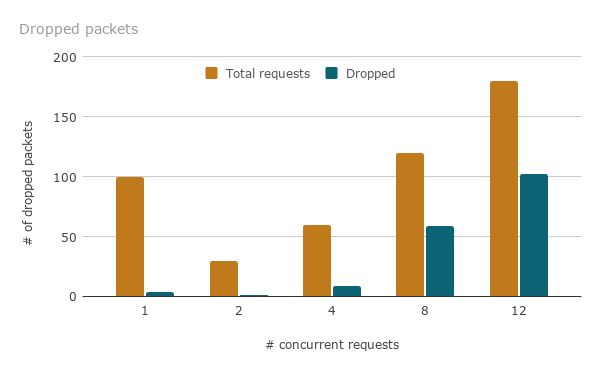
\includegraphics[width=\columnwidth]{figures/b-coap-2}
% \caption{Number of dropped packets as concurrency increases \label{fig:b-coap-2}}
% \end{figure}

% Fig. \ref{fig:b-coap-1} and Fig. \ref{fig:b-coap-2} present the experimental evaluation of the CoAP implementation in Rust. The STM32F407 is equipped with a LAN8720 ETH 10/100Mbs module connected to the microcontroller via cheap jumper wires. On the software stack, the device offers a CoAP server running on the RTIC runtime. Such a server is put under stress by firing concurrent requests from a machine connected to the same network, and the test is repeated 15 times. As expected, the response times increase as the number of concurrent requests rises. However, such escalation of response time is not exponential and presents a good smoother curve. The standard deviation range is also significantly large, as the embedded device cannot provide timely responses. Further experiments should compare the CoAP server with an equivalent HTTP or MQTT server running on the same RTIC runtime.

% On a different note, the number of dropped packets dramatically increases as the concurrency grows. Such behaviour is expected, and the experimental logs provide a plausible rationale. As the number of concurrent requests increases, the microcontroller network buffers cannot cope with the volume, and the packets are even truncated before being parsed. A deeper analysis should check whether the issue can be solved by allocating more buffer space or, on the contrary, is a hardware-related limit. Admittedly, the hardware network connection via jumper wires is not the most robust solution.

\subsection{Evaluation of Wasm as virtualisation technology}

The following benchmarks measure how long it takes to create and boot a Wasm-based Kubernetes Pod, how the memory scales as the number of running Pods increases, and how both metrics compare to containers. The benchmark is a simple DateTime application that logs the current system time upon creation and goes into sleep. By going to sleep, the Pod does not complete, and the resources remain allocated. The log is later retrieved using the Kubernetes API to calculate the boot time. 

Wasm Pods run on Krustlet \cite{krustlet}, whereas container Pods are scheduled on the K3s \cite{k3s} Kubelet. Krustlet (a Kubernetes-rust-kubelet) is an experimental implementation of the Kubelet APIs that supports Wasm as virtualisation technology. It is designed to run as a Kubernetes Kubelet. Therefore, it listens to the Kubernetes API event stream for new Pods and runs them under a WebAssembly System Interface (WASI) runtime (notably, Wasmtime by Mozilla \cite{wasmtime}).

On the other hand, K3s is a fully certified Kubernetes distribution geared towards resource-constrained environments backed by a commercial company. K3s is implemented in Go and packaged as a single binary of about 50MB in binary size. It bundles everything needed to run Kubernetes, including the container runtime (namely containerd \cite{containerd}), a Container Network Interface implementation (Flannel \cite{flannel}), a DNS server (CoreDNS \cite{coredns}), and a simple ingress load balancer (Traefik \cite{traefik}). The OS dependencies are also minimal and well supported by all the modern Linux distributions.

Krustlet has been customised to measure the time it starts to instantiate the Pod's necessary Wasm runtime. On the other hand, K3s and Kubernetes do not provide tools explicitly meant to obtain such value, and the author does not have the Go knowledge to modify and re-compile K3s. As a result, the start time is collected from the Kubernetes Pod metrics, which provides the time at which the Kubelet receives the request to provision the container. The provision request is followed by the container image's pull and then instantiation of the container itself. To avoid counting the additional image pull time, the author has explicitly configured the Pod to use the cached image and ensured that the Kubelet always has such cache. Lastly, the granularity of the Kubernetes start time metric is only up to seconds.

\begin{figure}[ht]
\centering
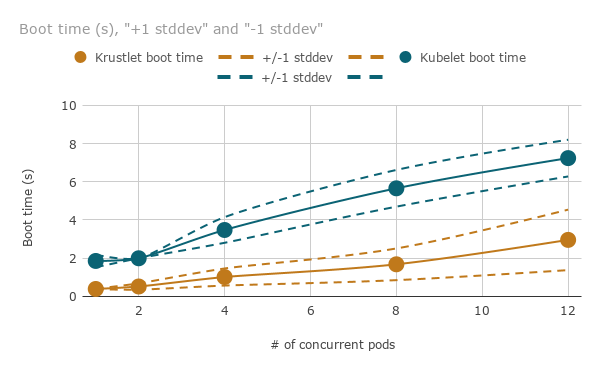
\includegraphics[width=\columnwidth]{figures/b-krustlet-1}
\caption{Average boot time for concurrent Wasm Pods \label{fig:b-krustlet-1}}
\end{figure}

Fig. \ref{fig:b-krustlet-1} shows the average boot time, along with the standard deviation, of both the Kubernetes Pods containing Wasm binaries and the conventional Pods containing containers. The benchmark concurrently deploys the Pods and repeats the process 15 times. Pods are not deleted between iterations, so that memory utilisation is also collected.

The experimental results show that a Wasm-based virtualisation strategy incurs less boot time. However, the more mature container Kubelet presents a more linear curve and minor standard deviation as the number of concurrent deployments increases. Because efficient concurrency is essential as much as a fast boot time, there is no clear winner. Nevertheless, such preliminary results encourage the idea of adopting Wasm as an alternative to container technology since efficiency was not a primary design goal in the early implementations of Krustlet and Wasmtime. Future versions will probably provide even more competitive results.

\begin{figure}[ht]
\centering
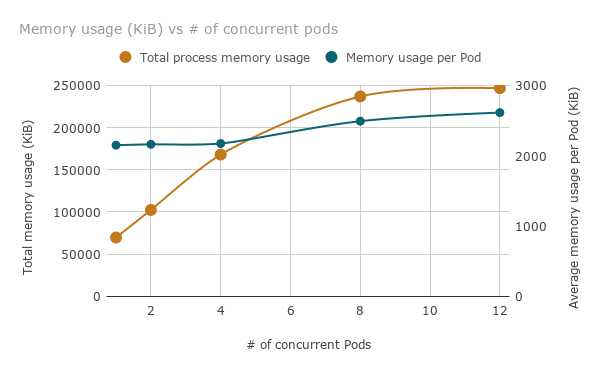
\includegraphics[width=\columnwidth]{figures/b-krustlet-2}
\caption{Average memory usage of concurrent Wasm Pods \label{fig:b-krustlet-2}}
\end{figure}

\begin{figure}[ht]
\centering
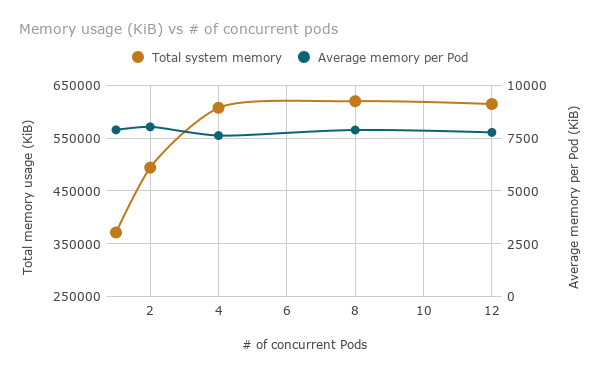
\includegraphics[width=\columnwidth]{figures/b-krustlet-3}
\caption{Average memory usage of concurrent K3s Kubelet Pods \label{fig:b-krustlet-3}}
\end{figure}

Fig. \ref{fig:b-krustlet-2} and Fig. \ref{fig:b-krustlet-3} offer an overview of the memory overhead of the two different virtualisation solutions. The memory utilisation has been tracked using the Linux \emph{pmap} utility, which allows the granular analysis of the system memory allocated by a process. In Krustlet's case, the task is trivial as Wasm modules run in the same process as the host, and only additional Pods can significantly increase the heap memory, as Rust is not garbage collected. On the contrary, K3s instantiates a process for each new container. It is much more difficult to evaluate each Pod's memory cost, as the Go language uses the heap for every aspect. Therefore, in the latter case, we resort to measuring the system memory using the Linux \emph{free} program. Fortunately, since the author uses Alpine Linux with a minimal configuration to support just enough to run Kubernetes, the system measurements are relatively free from other processes' contamination.

In such a comparison, Wasm Pods are the winners in memory usage per Pod unit, but the K3s Kubelet can achieve higher total memory utilisation. Notably, the K3s Kubelet can completely use the available memory until the machine cannot even function properly. On the other hand, the Krustlet node fails to allocate new Pods even when there is sufficient memory space. The allocation results in an Out Of Memory error, and the node is still completely functional. To the best of the author's knowledge, the potential cause is the Rust vector allocation strategy, which doubles the capacity when its current limit is reached. As a result, when Krustlet's heap reaches about 256MB, the process demands the kernel an additional 512MB of space. Such demand cannot be met, and the Rust runtime returns an Out Of Memory error. Further analysis of the Wasmtime implementation is needed to validate this hypothesis. 

On a different note, as Go is a garbage-collected language, the heap utilisation is highly unpredictable. The Go Garbage Collector (GC) uses a pacer to determine when to trigger the next GC cycle \cite{go-gc}. Pacing is modelled like a control problem where it is trying to find the right time to trigger a GC cycle to hit the target heap size goal. Go’s default pacer will try to trigger a GC cycle every time the heap size doubles. The net result is that the K3s increase memory usage even during idle periods, as it processes the ordinary Kubernetes operations to maintain functionality. Besides, as the GC kicks in only when the heap size doubles, the hardware memory is underutilised. The freeable memory should be used for running additional pods, achieving better Pod packing. Such efficiency is crucial for edge nodes that have already limited hardware capabilities but must support multiple workloads. This consideration is another point favouring the adoption of the Rust language to develop the continuum infrastructure. Table \ref{tab1} presents the system memory utilisation during an idle state.

Lastly, in both technologies, the memory overhead per Pod is relatively constant. However, the Wasm Pod incurs approximately 2x-3x less overhead, allowing more efficient packing of applications on the same machine. For example, the Raspberry Pi 3B+ can support up to 80 Wasm Pods and still have 500MB of free memory (although no more Pods can be allocated). In contrast, the K3s Kubelet achieves maximum memory utilisation of about 55 container Pods, and the entire node becomes completely unresponsive. The author believes that such results pledge to favour Krustlet, as the premature Out Of Memory error can be fixed on later Wasmtime versions. In contrast, the container overhead is already the state of the art of a decade of research in container technologies.

\begin{table}
\caption{Memory usage of Kubernetes on edge Raspberry Pi}
\begin{tabular}{|l|l|}
\hline
Software stack & Idle memory usage \\
\hline
Alpine Linux 3.12.1 & ~50MB \\
Alpine Linux + K3s master & ~304MB \\
Alpine Linux + K3s agent & ~110MB \\
Alpine Linux + Krustlet & ~120MB \\
\hline
\end{tabular}
\label{tab1}
\end{table}

\subsection{Evaluation of Wasm for Machine Learning}

In the field of machine learning, numerical precision matters. WASM natively supports floating-point arithmetic, whereas other popular machine learning backends like WebGL requires hardware extensions. Not all devices support this extension, which means a GPU-accelerated machine learning is not supported on some devices (e.g. older mobile devices which can run Wasm instead).

Moreover, GPU drivers can be hardware-specific and different devices can have precision problems. On iOS, 32-bit floats are not supported on the GPU. Consequently, TensorFlow \cite{tensorflow}, the popular machine learning library developed by Google, falls back to 16-bit floats, causing precision problems. In WASM, computation always happens in 32-bit floats and thus have precision parity across all devices. Such numerical predictability is also paramount in blockchain applications, as proved by Parity's interest in WebAssembly \cite{parity-wasm}.

The author has compiled the flood prediction model to Wasm, and Fig. \ref{fig:b-krustlet-4} evaluates the model's response time with increasing concurrency. The flood prediction model is a conventional Deep Neural Network constituted by three dense layers of 32, 16 and 1 units. The model has been trained on the cloud using the traditional machine learning framework Keras \cite{keras}. Keras provides a Python interface for artificial neural networks on top of the TensorFlow library.

As of the time of writing, TensorFlow provides a WebAssembly (WASM) backend for both the browser and Node.js \cite{tf-wasm}. However, the library itself cannot be easily compiled to WebAssembly yet, to the best of the author's knowledge. As a result, the trained Keras model is saved to the ONNX \cite{onnx} standard format and executed by the \emph{tract} library \cite{tract}. tract is a Rust neural network inference library that can read Tensorflow or ONNX models and run data through them. It also supports compilation to Wasm as a target. The resulting Wasm module exports a public function through which Krustlet can pass the model inputs. 

At the time of writing, it has not been possible to implement a web server directly on top of the inference model and compile the application to Wasm. There is an underlying issue with implementing network servers with Wasm as there is neither complete network nor multi-threading support yet.

First, the current WebAssembly System Interface (WASI) standard only contains a few methods for working with sockets that are not enough for complete networking support. Adding support for connecting to sockets is fundamental to allow Wasm modules to connect to web servers, databases, or any service. As a workaround, this paper has implemented the capability to invoke functions in Wasm Pods on top of the Kubernetes \emph{exec} API \cite{k8s-exec}, which is however designed to execute commands in a container from the Kubernetes command line, and it is an undocumented interface. Besides, as WASI lacks network APIs and Krustlet does not support the Kubernetes networking configuration yet, the POC uses a hybrid approach where conventional Kubelets with container runtimes are used as a fallback.

Second, the lack of concurrency primitives means that a server running in WebAssembly is single-threaded, or its implementation has to be significantly more complex (e.g. Node.js's event loop). This limitation severely narrows the workload capabilities of the server. At the time of writing, the WASM spec has outlined a thread and atomics proposal intending to speed up multi-threaded applications. The proposal is still in the early stage, and it is implemented only in web browsers, behind an experimental flag.

\begin{figure}[ht]
\centering
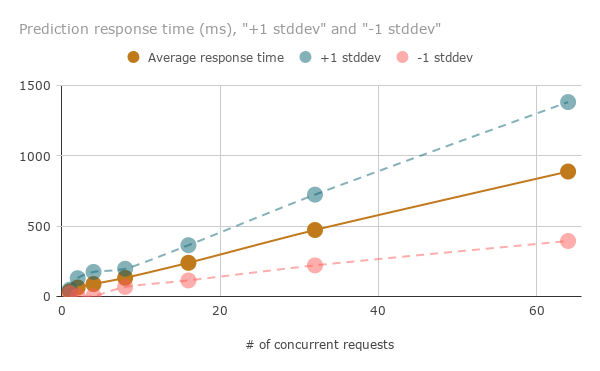
\includegraphics[width=\columnwidth]{figures/b-krustlet-4}
\caption{Latency of the Wasm flood prediction model with varying concurrency \label{fig:b-krustlet-4}}
\end{figure}

Fig. \ref{fig:b-krustlet-4} illustrates the flood prediction response times within a Wasm Pod in the same fashion of serverless functions. As expected, the response times increase linearly with varying concurrency. Because the WASI standard does not support multi-threading, the requests are completed sequentially.

\section{Conclusion}
\label{sec:conclusion}

This paper has presented a computing continuum vision and the challenges that the industrial and academic community will face implementing such a paradigm. The author has also presented an effort to suggest a potential architecture for the infrastructure and implemented a Proof of Concept of such architecture based on the technologies available at the time of writing. Such POC has been applied to a real-world use case of flood prediction as well. The net result is a working prototype based on the presented architectural and software concepts. The implementation is publicly available on GitHub \cite{fedra-thesis}. 

In the author's view, we are clearly at a convergence point after the last decades of technological advances. The computation must be free to flow in the continuum between the ends of the network. However, a significant number of challenges (§\ref{sec:challenges}) lie ahead, and an even greater effort from all the stakeholders is required.

The WebAssembly standard is a potential enabling technology for the realisation of the continuum, but it is still in its infancy. As shown by the experimental results, WebAssembly is mainly suited for pure computational functions. The lack of multi-threading and a mature network interface severely limit the space of real-world applications. Most of the production use cases of WebAssembly involve pure computation scenarios, typically machine learning and relatively simple serverless functions. Other projects like wasmcloud \cite{wasmcloud} (previously named wasCC) try to overcome the API limitations by providing custom system capabilities, to the detriment of the platform-independency feature of WebAssembly, unfortunately.

% However, it is undeniable that the Wasm bytecode format has attracted interest from multiple parties like Cloudflare, Fastly, and Parity, despite WebAssembly was initially conceived for efficient execution in a browser context. These commercial companies are interested in its performance, portability and sandboxing capabilities for different scopes than browser execution. Other companies, namely Mozilla, Intel, Red Hat and Fastly again, have joined the efforts to the birth of the Bytecode Alliance \cite{bytecode-alliance}. As stated by the members, the official goal of the alliance is to "establish a capable, secure platform that allows application developers and service providers to confidently run untrusted code, on any infrastructure, for any operating system or device, leveraging decades of experience doing so inside web browsers."

% Seeing such public announcements from notorious industry leaders may bring excitement at first, but it is hard to state if such commitment is real or just a side project between many. In August 2020, Mozilla laid off most of its employees \cite{mozilla-lies-off}, notably the whole Wasm team and a large slice of the Rust core team. Many developers have been employed by other companies interested in Rust and Wasm, e.g. Fastly and Amazon. However, it is hard to tell if they will be able to maintain the commitment. For example, active development of wasm-bindgen \cite{wasm-bindgen} has ceased, even though wasm-bindgen is the most popular tool for high-level interaction between Wasm and the JavaScript browser runtime.

% This evident interest pattern but lack of financial and stable support from commercial companies is typical in WebAssembly and Rust. Companies are still gaining interest in hiring Rust developers \cite{aws-rust} to modernise their existing infrastructure rather than committing to new technologies like WebAssembly. For example, despite Intel being part of the Bytecode Alliance and author of a Wasm runtime for microcontrollers (wasm-micro-runtime \cite{wasm-micro-runtime}), there has not been progress in discussing and proposing memory pages smaller than 64KiB in the WebAssembly standard, despite the issue being well-known for years \cite{wasm-64}.

% Microsoft has been notably providing more financial support compared to the other cloud providers. The development of both the Krustlet project and the Akri project is lead by developers of the Deis Labs team \cite{deislabs}, whose members maintain several vital projects in the cloud community (notably Helm, the package manager for Kubernetes). As a result, the future perspective for Krustlet and Akri is brighter than other projects like wasm-bindgen. Both projects are still highly immature, but they are expressive in depicting the future direction of Wasm and Kubernetes as critical technologies of the computing continuum.

Results show that Wasm-based Pods in Krustlet incur fixed low overhead in memory usage and competitive boot times compared to more mature container solutions. The outcome is intriguing as these technologies (Krustlet and Wasmtime) are still in their infancy.

As a concluding note, although the proposed architecture and the related technologies are still very immature, they open up a set of exciting opportunities for the continuum's realisation.
